\documentclass[aspectratio=169, 12pt, compress]{beamer}

\usepackage[bgphoto]{Configuration_Files/beamerthemepolimi}

% Full instructions available at:
% https://github.com/elauksap/beamerthemepolimi

% Set custom font (requires to compile with XeLaTeX).
\usepackage{ifxetex}
\ifxetex
    \usepackage{fontspec}
    \setsansfont[Scale=0.95]{Arial}
\fi

% STANDARD MATH PACKAGES
\usepackage{amsmath}
\usepackage{amsthm}
\usepackage{bm}
%\usepackage[overload]{empheq}  % For braced-style systems of equations

% REFERENCES PACKAGES
\usepackage[capitalize]{cleveref}

% COLOR
\usepackage{xcolor}

% IMAGES AND TABLES
\usepackage{wrapfig}
\usepackage{tabularx}
\usepackage{longtable}
\usepackage{colortbl}
\usepackage{multirow}
\usepackage{hhline}
\usepackage{makecell}

\newcommand{\gbm}[1]{\bm{\mathbf{#1}}} % General Bold Math for both greek and latin letters
\newcommand{\rowcolorhang}[1]{\rowcolor{#1}[\dimexpr\tabcolsep+0.1pt\relax]} % Add overang to table row coloring, to avoid vertical white lines
\creflabelformat{equation}{#2\textup{#1}#3} % Remove parentheses from cleveref equations
\newcommand{\T}{\mathrm{T}} % Transpose
\newcommand{\overimage}[2][0cm]{\vspace{#1}\vfill\smash{\begin{minipage}[c][][c]{\linewidth}\centerline{#2}\end{minipage}}\vfill} % Minipage container for images in overprint

\makeatletter
\patchcmd{\beamer@sectionintoc}
  {\vfill}
  {\vskip\itemsep}
  {}
  {}
\makeatother

\title{Interpreting Large Language Models Through the Lens of Embedding-Oriented Visualizations}
\subtitle{Markov Models, Sankey Diagrams and Comparative Approaches}
\author{Davide Rigamonti}
\advisor{Prof. Mark Carman}
\coadvisors{Nicolò Brunello, Vincenzo Scotti}
\date{03/04/2025}

\begin{document}

    \begin{frame}
        \maketitle
        % If the theme option "nologo" is specified, a custom logo
        % can be added with the following commands:
        %\begin{tikzpicture}[overlay, remember picture]
        %    \node at (current page.north) [anchor=north, inner sep=2cm]
        %    {
        %        
\includegraphics[width=0.3\paperwidth]{logo_centrato_BN_negativo.png}
        %    };
        %\end{tikzpicture}
    \end{frame}
    
    \begin{frame}{Table of Contents}
        \setcounter{tocdepth}{2}
        \vspace{0.2cm}
        \begin{columns}[onlytextwidth,T]
            \hfill%
            \begin{column}{.35\textwidth}%
                \tableofcontents[sections=1-3]%
            \end{column}%
            \hfill%
            \begin{column}{.35\textwidth}%
                \tableofcontents[sections=4-6]%
            \end{column}%
            \hfill%
        \end{columns}
    \end{frame}
    
    \section{Introduction}

    \subsection{Background}

    \begin{frame}{Transformer Architecture and Embeddings}
        \begin{minipage}{0.55\textwidth}
            \centering%
            \begin{overprint}%
                \onslide<1>
                \overimage[0.25cm]{\includegraphics[width=0.82\textwidth]{pres_drw_transformer-1.pdf}}%
                \onslide<2>
                \overimage[0.25cm]{\includegraphics[width=0.74\textwidth]{pres_drw_transformer-2.pdf}}%
                \onslide<3>
                \overimage[0.25cm]{\includegraphics[width=0.99\textwidth]{pres_drw_embedding.pdf}}%
                %\onslide<4>
                %\overimage[0.25cm]{\includegraphics[width=0.6\textwidth]{background_embeddings.pdf}}%
            \end{overprint}%
        \end{minipage}%
        \begin{minipage}{0.45\textwidth}
            \footnotesize
            \begin{itemize}[<+|visible@+->]
                \setlength\itemsep{0.05cm}
                \item<1-1> \emph{Language models (LMs)} generate text word-by-word by guessing the next word (token) given the previous context.
                \item<1-1> The basic Transformer block features \emph{Feed-Forward Neural Network (FFNN)} and \emph{attention} components with additive contributions to the residual flow.
                \item<2-2> Transformer-based LMs use replicated blocks to manipulate vector representations through multiple steps (layers).
                \item<3-3> These hidden state vectors form the \emph{`internal language'} of the model, translated through the \emph{embedding} and \emph{LM head} blocks.
            \end{itemize}
        \end{minipage}
    \end{frame}

    \subsection{Research Questions}

    \begin{frame}{Hidden State Visualization}
        \begin{minipage}{0.8\textwidth}
            \begin{itemize}[<+|visible@+->]
                \setlength\itemsep{0.6cm}
                \item \textbf{Question 1:} How can we visualize internal states of LLMs in an immediate and interactive way?
                \item \textbf{Proposed Solution:} Development of an interactive visualization tool for LLMs, \emph{InTraVisTo (Inside Transformer Visualization Tool)}, designed to support machine learning researchers in hypothesis formulation by offering a unique perspective on the internal representations of LLMs.
            \end{itemize}
        \end{minipage}%
        \begin{minipage}{0.2\textwidth}
            \centering%
            \includegraphics[width=0.72\textwidth]{pres_drw_transformer-single.pdf}%
        \end{minipage}%
    \end{frame}

    \begin{frame}{Linearity in the Embedding Space}
        \begin{minipage}{0.8\textwidth}
            \begin{itemize}[<+|visible@+->]
                \item<1-1> \textbf{Question 2:} Do autoregressive LLMs retain linear properties in their embedding spaces?
                \item<2-3> \textbf{Proposed Solution:} Use experiments based on analogies to assess the relationship between distance and semantic/morphological similarity on the embedding spaces of recent models.
                \begin{itemize}[<+|visible@+->]
                    \item<3-3> Identify key differences in the embedding spaces generated by classic transformer architectures against autoregressive LLMs.
                    \item<3-3> Clarify how the shift from the input representation to the output one affects the embedding spaces involved through the layers of an LLM.
                \end{itemize}
            \end{itemize}
        \end{minipage}%
        \begin{minipage}{0.2\textwidth}
            \centering%
            \includegraphics[width=0.81\textwidth]{background_emb-arithmetic_placeholder.pdf}%
        \end{minipage}%
    \end{frame}

    \begin{frame}{First-Order Predictions from Embeddings}
        \begin{minipage}{0.8\textwidth}
            \begin{itemize}[<+|visible@+->]
                \item<1-1> \textbf{Question 3:} Is it possible to obtain first-order predictions by concatenating embedding spaces in LLMs?
                \item<2-3> \textbf{Proposed Solution:} Compare a trained bigram Markov model and an identity matrix against the transition matrix of a First Order Model (FOM) obtained by multiplying the embedding and unembedding matrices of an LLM.
                \begin{itemize}[<+|visible@+->]
                    \item<3-3> Evaluate similarity or dissimilarity between the transition matrices using direct matrix comparison and set similarity metrics.
                    \item<3-3> Evaluate similarity or dissimilarity between the transition matrices using probabilistic metrics such as perplexity and KL divergence.
                \end{itemize}
            \end{itemize}
        \end{minipage}%
        \begin{minipage}{0.2\textwidth}
            \centering%
            \includegraphics[width=0.8\textwidth]{pres_drw_fom.pdf}%
        \end{minipage}%
    \end{frame}

    \section{State of the Art}

    \begin{frame}{Vocabulary Space Decoding}
        \begin{minipage}{0.48\textwidth}
            \centering
            {\justifying\footnotesize \emph{Logit Lens} is one of the first \textbf{vocabulary space decoding} implementations, involving the decoding of interlayer hidden representation using the model's own unembedding matrix. \\[2pt]}
            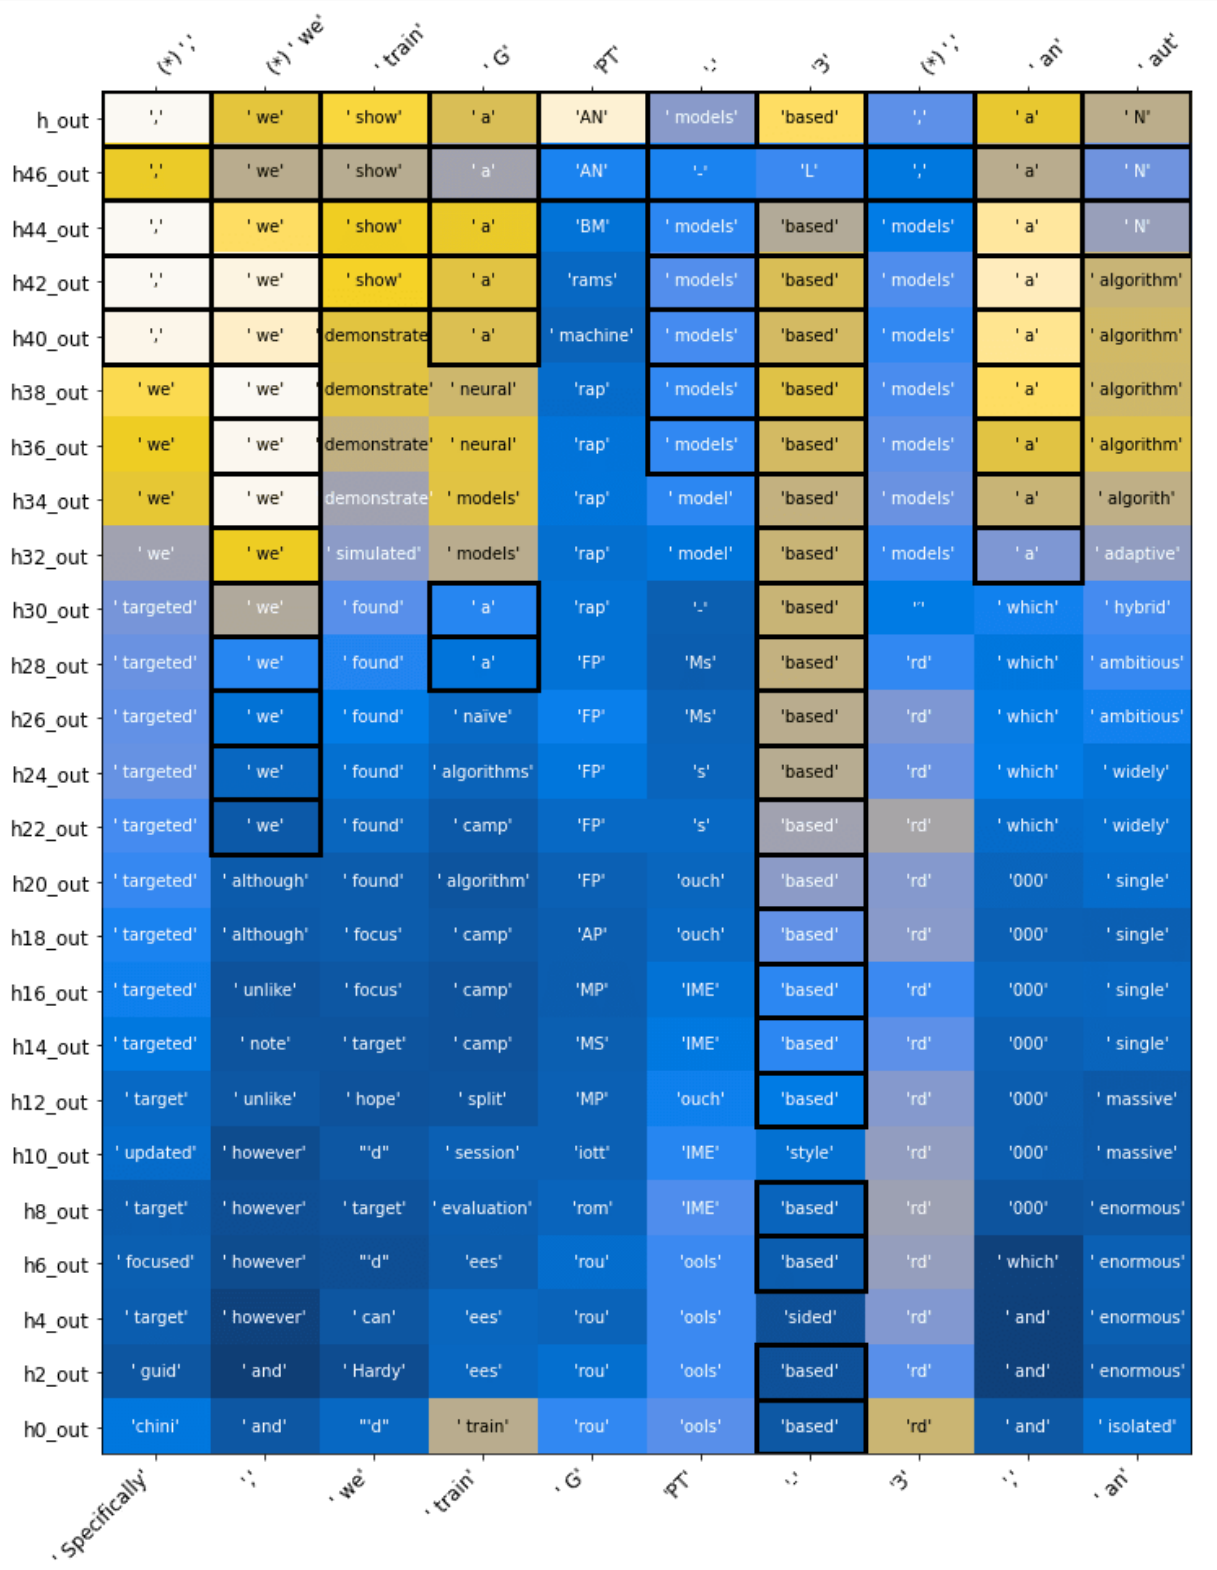
\includegraphics[width=0.49\textwidth]{logit-lens.png}
        \end{minipage}%
        \hfill%
        \begin{minipage}{0.48\textwidth}
            \centering
            {\justifying\footnotesize \emph{LM Transparency Tool (LM-TT)} builds on top of the circuital interpretation of the Transformer to visualize the information flow, focusing on the attention paths, and providing useful decoding information. \\[2pt]}
            \includegraphics[width=0.75\textwidth]{related_lm-tt.pdf}
        \end{minipage}
    \end{frame}

    \section{Transformer Visualization}

    \subsection{Explorative Analysis}

    %\begin{frame}{InTraVisTo}
    %    \begin{minipage}{0.75\textwidth}
    %        \begin{itemize}[<+|visible@+->]
    %            \item<1-1> InTraVisTo allows decoding and inspection of the \emph{main four vectors} that compose each layer of the Transformer architecture.
    %            \item<2-2> The vectors correspond to the output of the attention component ($\gbm{\delta}_{\textit{att}}^{(\ell)}$), the intermediate state (${\gbm{x}'}^{(\ell)}$) given by the addition of the attention component to the residual stream, the output of the feed-forward network component ($\gbm{\delta}_{\textit{ff}}^{(\ell)}$), and the layer output ($\gbm{x}^{(\ell)}$).
    %            \item<3-3> The decoding operation is carried out using a specialized decoder which, given a hidden state as input, finds related tokens from the model's vocabulary with the goal of returning an interpretable output.
    %        \end{itemize}
    %    \end{minipage}%
    %    \begin{minipage}{0.25\textwidth}
    %        \centering
    %        \includegraphics[width=0.7\textwidth]{placeholder_pres_transformer.png}%
    %    \end{minipage}
    %\end{frame}

    \begin{frame}[empty]{}
        \vspace*{-0.15cm}
        \only<1-2>{
            \begin{tikzpicture}
                \hspace*{-0.4cm}%
                \only<1>{\node[inner sep=0] (img) {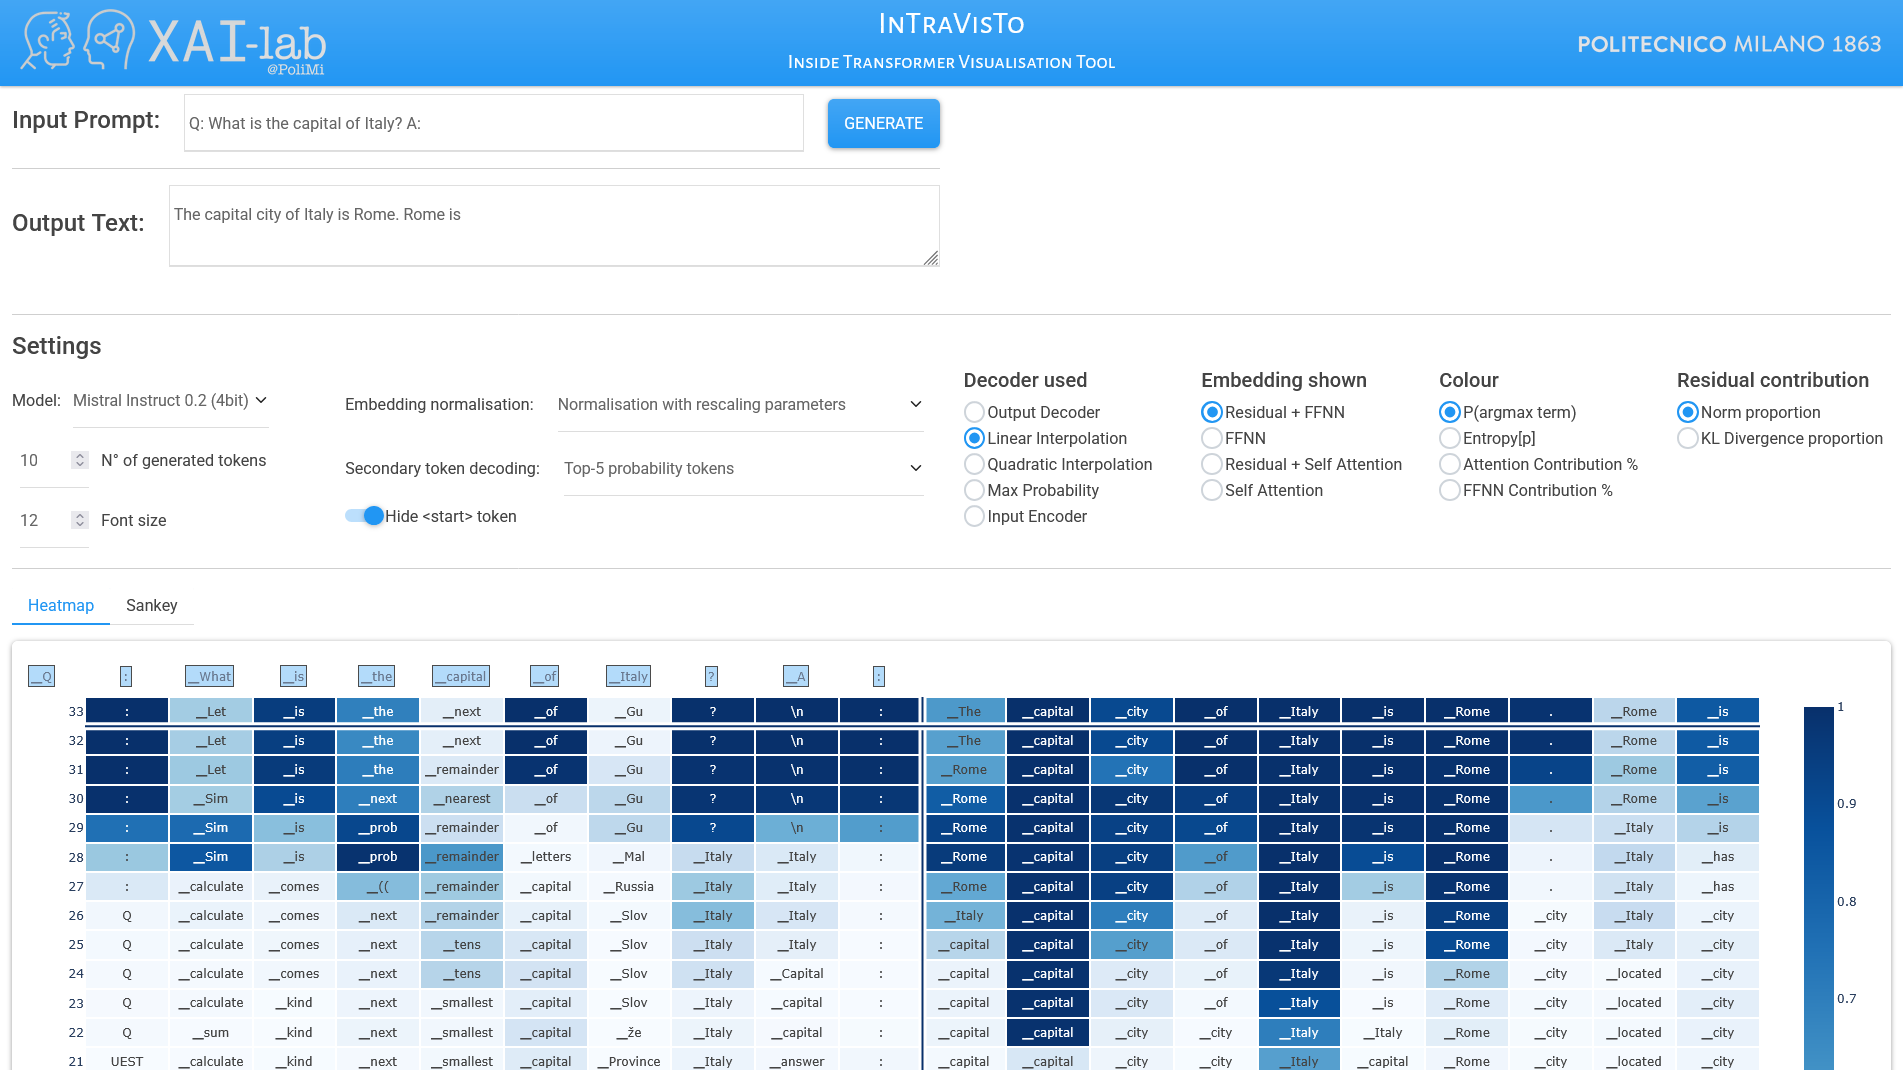
\includegraphics[width=\paperwidth]{pres_intravisto-interface.png}};}%
                \only<2>{\node[inner sep=0] (img) {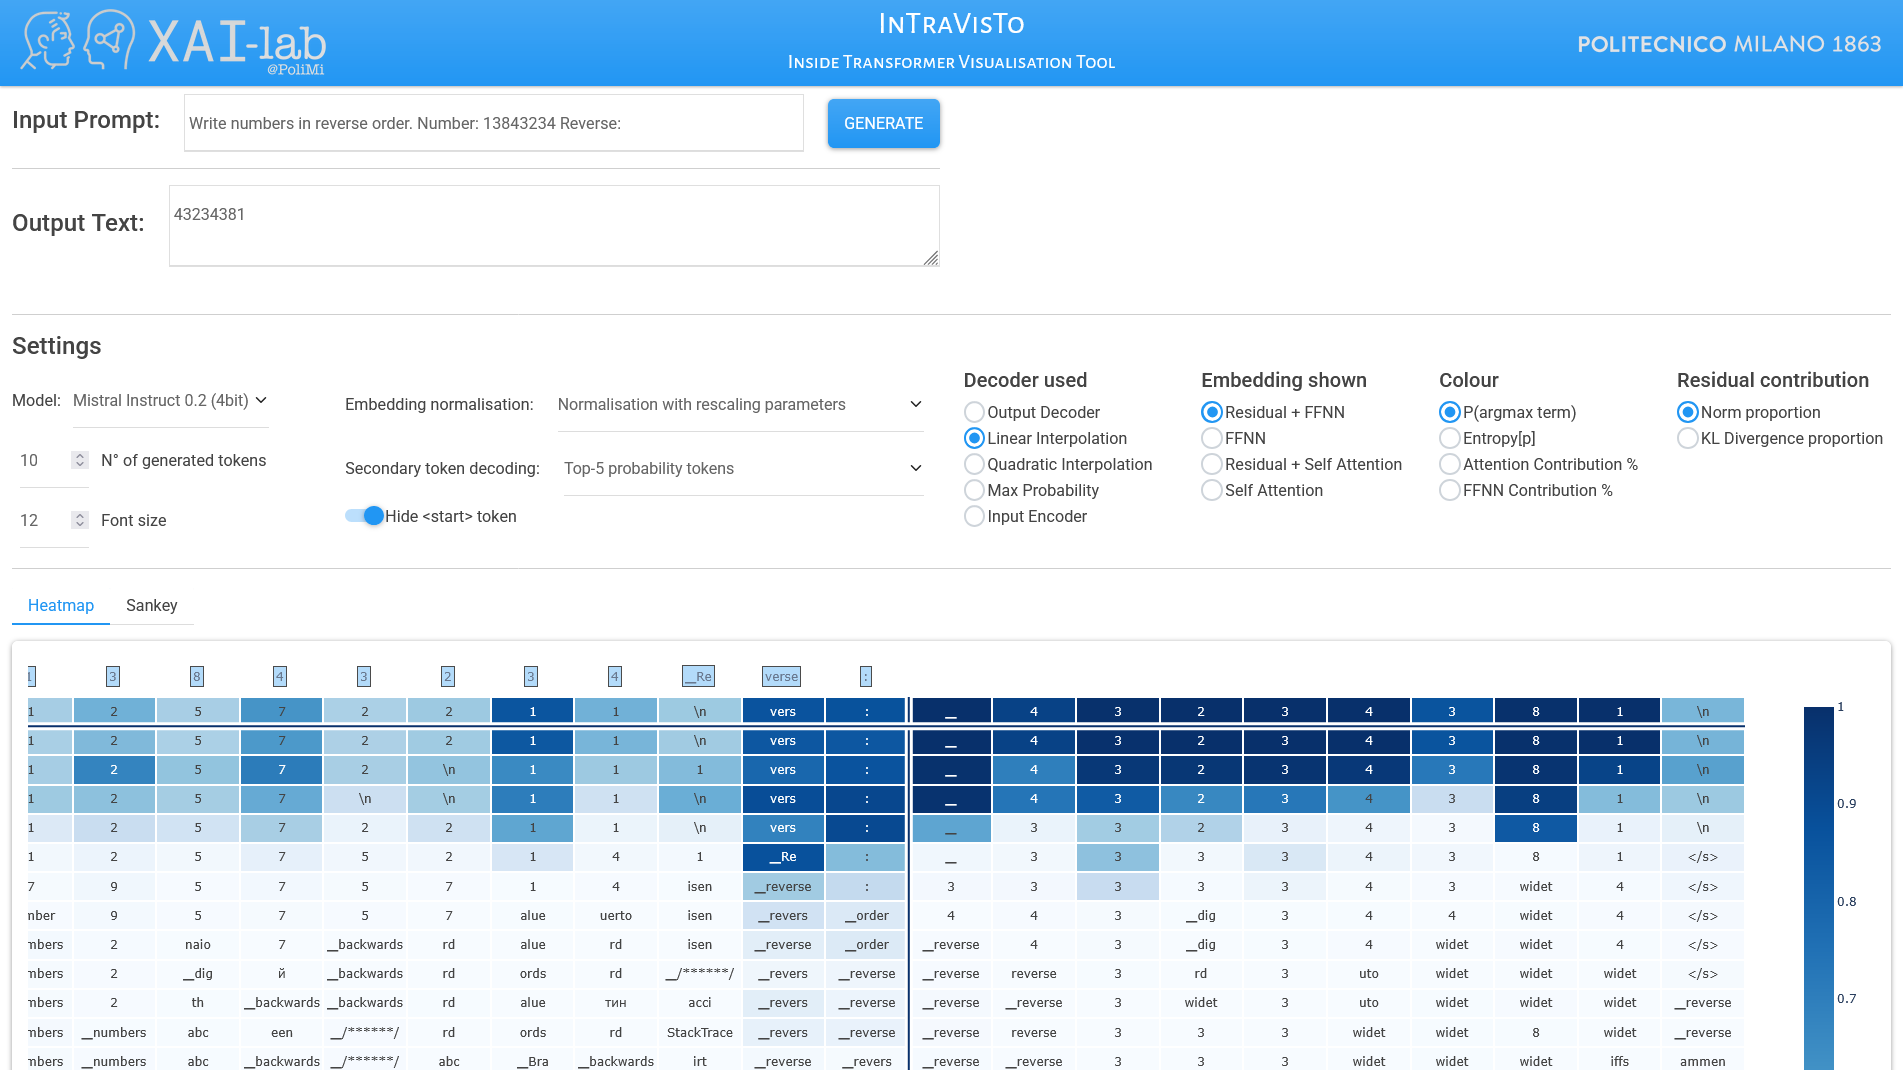
\includegraphics[width=\paperwidth]{pres_intravisto-example.png}};}%
                \only<2>{\draw[color=red,thick] (-7.98,2.2) rectangle (-0.04,3.75);}
            \end{tikzpicture}%
        }%
    \end{frame}

    \begin{frame}{Reverse Order Prompt}
        \begin{minipage}{0.6\textwidth}
            \centering
            \begin{overprint}%
                \onslide<1-2>
                \overimage{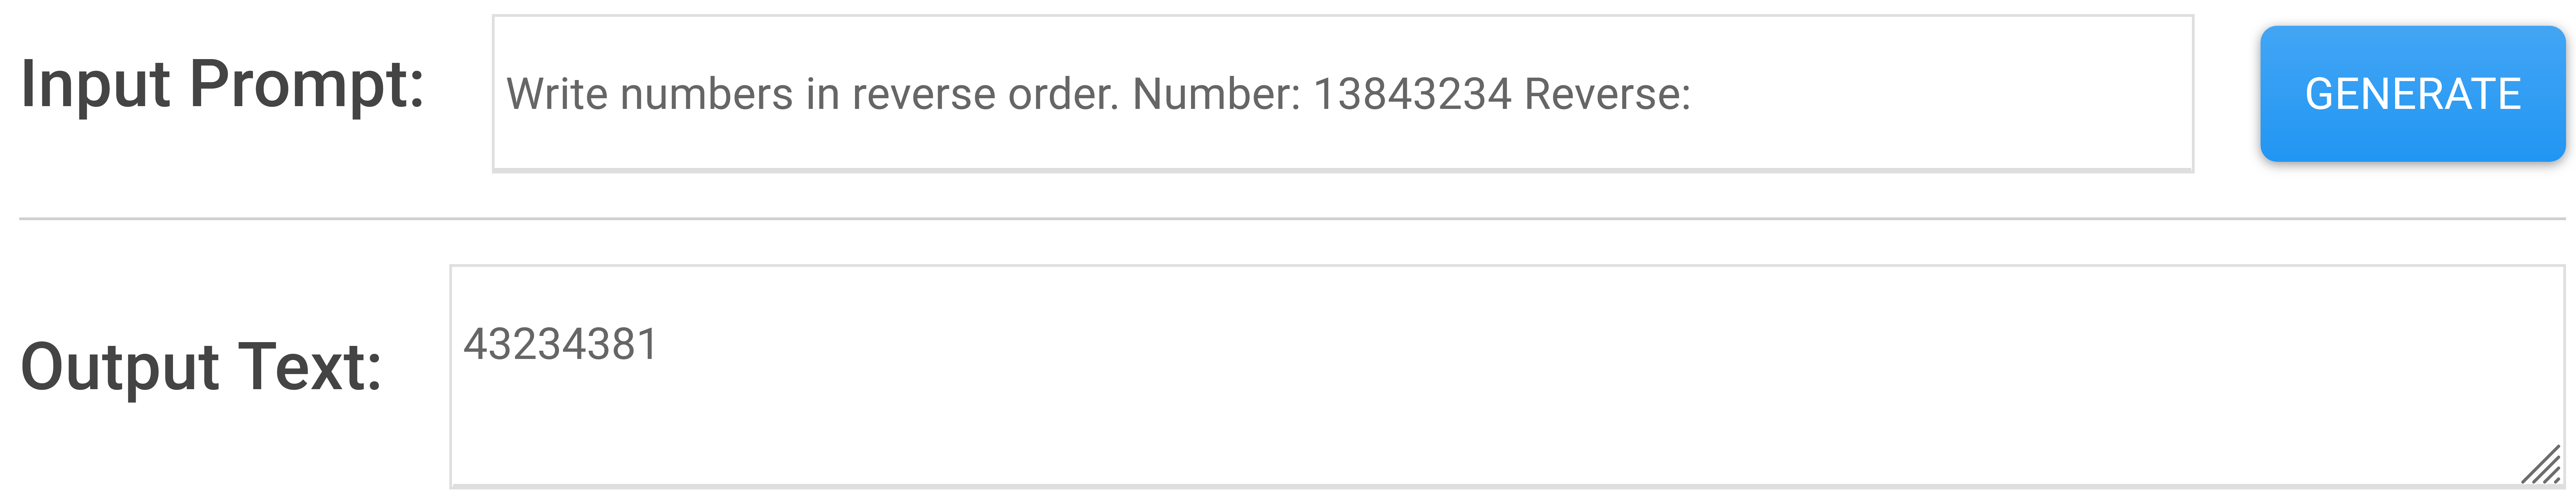
\includegraphics[width=0.95\textwidth]{exp_intravisto_4G_output.png}}%
            \end{overprint}%
        \end{minipage}%
        \begin{minipage}{0.4\textwidth}
            \footnotesize
            \begin{itemize}[<+|visible@+->]
                \setlength\itemsep{0.8cm}
                \item<1-1> Prompt Mistral model with the following query: \emph{``Write numbers in reverse order. Number: 13843234 Reverse:''}.
                \item<2-2> The returned answer is almost correct, two digits appear inverted ($3$ and $8$).
            \end{itemize}
        \end{minipage}
    \end{frame}

    \subsubsection{Decoding Interface}

    \begin{frame}[empty]{}
        \vspace*{-0.15cm}
        \begin{tikzpicture}
            \hspace*{-0.4cm}
            \node[inner sep=0] (img) {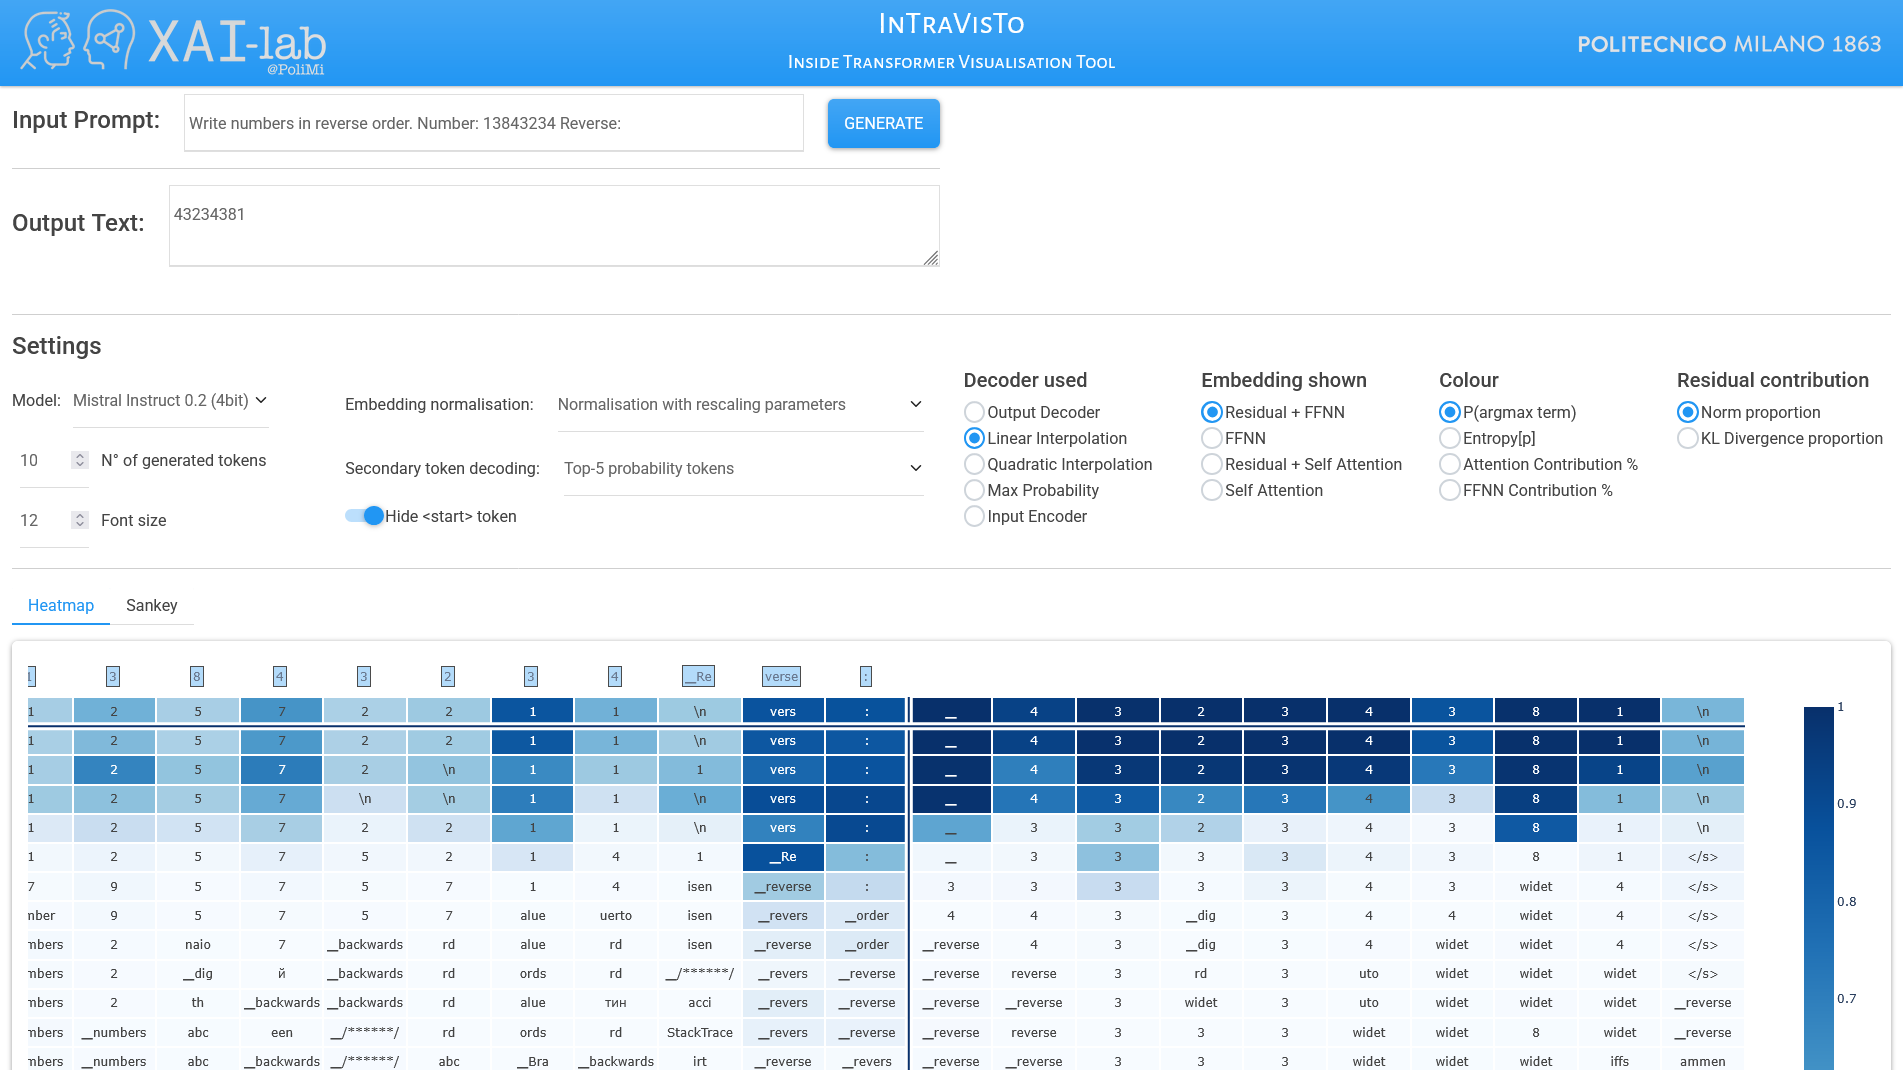
\includegraphics[width=\paperwidth]{pres_intravisto-example.png}};
            \draw[color=red,thick] (-0.4,-4.48) rectangle (6.7,-1.32);
        \end{tikzpicture}%
    \end{frame}

    \begin{frame}{Decoding States}
        \begin{minipage}{0.6\textwidth}
            \centering
            \begin{overprint}%
                \onslide<1-2>
                \overimage[0.4cm]{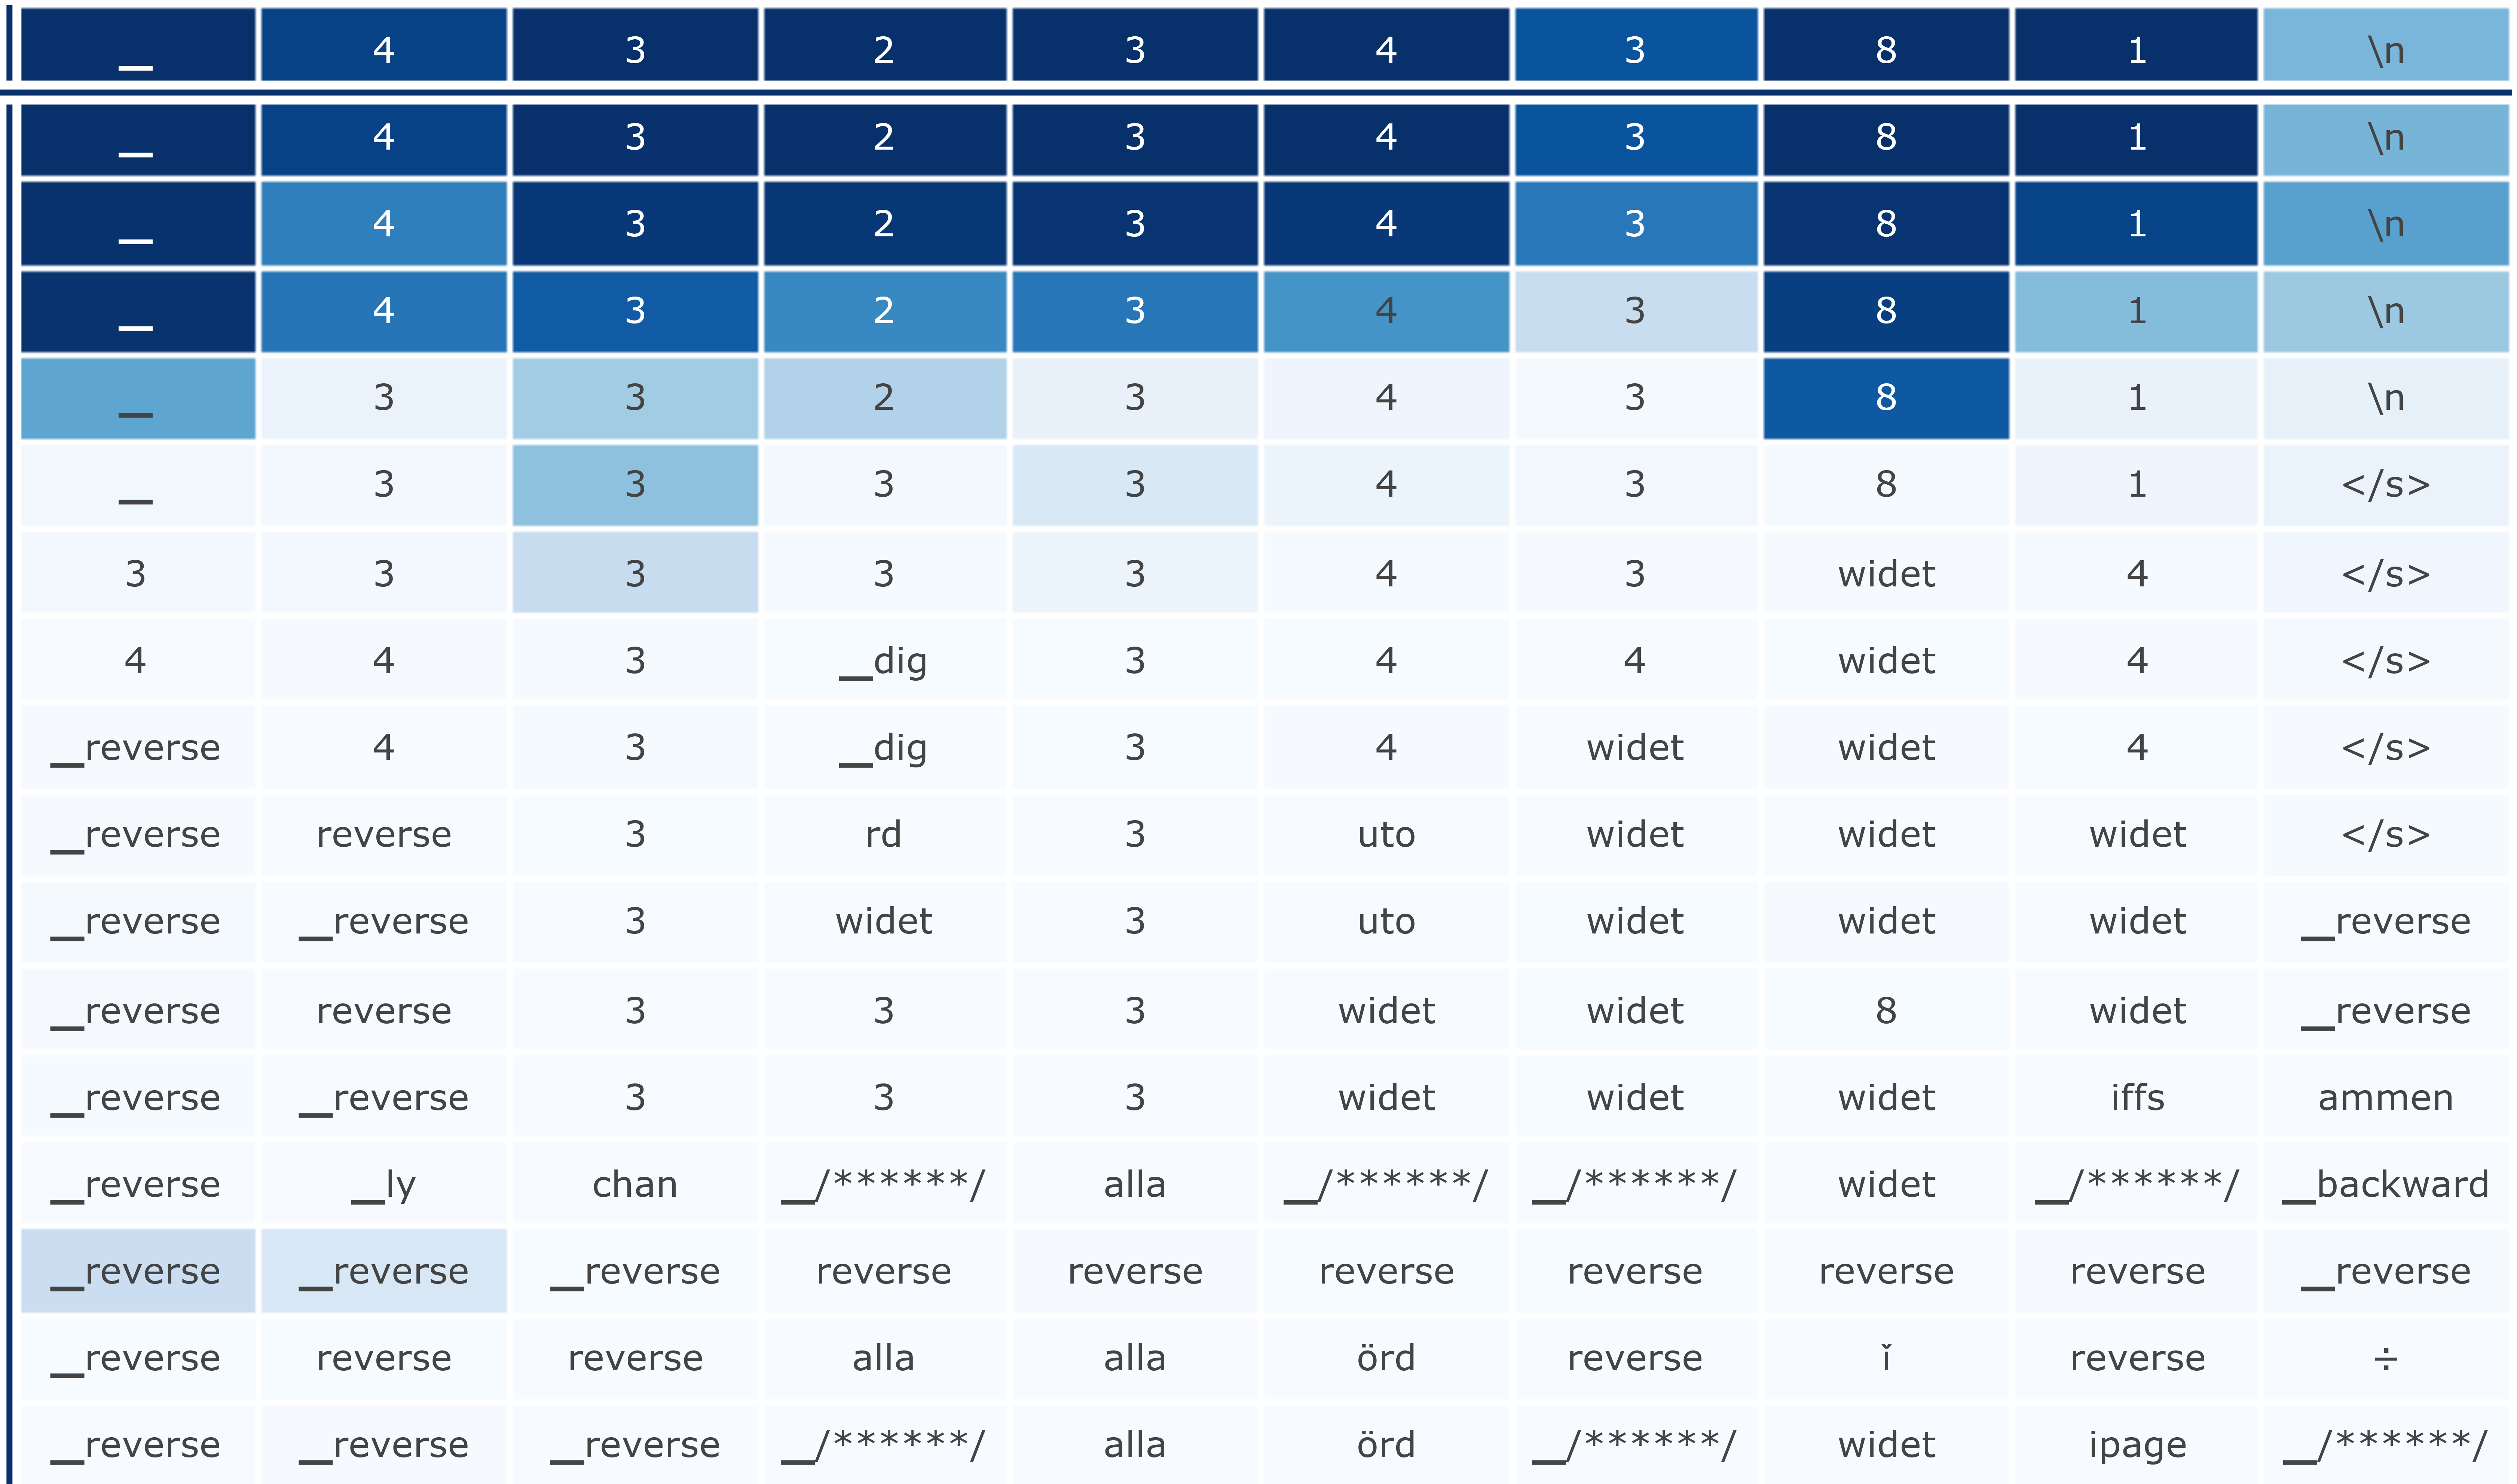
\includegraphics[width=0.95\textwidth]{exp_intravisto_4G_heatmap.png}}%
            \end{overprint}%
        \end{minipage}%
        \begin{minipage}{0.4\textwidth}
            \footnotesize
            \vspace*{0.3cm}
            \begin{itemize}[<+|visible@+->]
                \setlength\itemsep{0.3cm}
                \item<1-1> Decoding the meaning of hidden state vectors at various depths of a Transformer stack is essential for providing an intuition as to how the model is working.
                \item<2-2> Each cell represents a token-layer combination containing the main decoded hidden state in token form alongside its probability as the heatmap color.
                \scalebox{0.8}{\parbox{\textwidth}{%
                \begin{equation*}
                \begin{aligned}
                    P(\ \cdot \mid \gbm{x}, d_{\textit{dec}}, n_{\textit{norm}}) &= P(\ \cdot \mid \gbm{x}, \gbm{W}_{d_{\textit{dec}}}, N_{n_{\textit{norm}}}) \\
                    &= \operatorname{softmax}\Bigl(N_{n_{\textit{norm}}}(\gbm{x}) \cdot \gbm{W}_{d_{\textit{dec}}}\Bigr)
                \end{aligned}
                \end{equation*}}}
            \end{itemize}
        \end{minipage}
    \end{frame}

    \begin{frame}{Decoding States}
        \begin{minipage}{0.6\textwidth}
            \centering
            \begin{overprint}%
                \onslide<1-2>
                \overimage[0.5cm]{\includegraphics[width=0.8\textwidth]{pres_drw_embedding.pdf}}%
            \end{overprint}%
        \end{minipage}%
        \begin{minipage}{0.4\textwidth}
            \footnotesize
            \vspace*{0.3cm}
            \begin{itemize}[<+|visible@+->]
                \setlength\itemsep{0.3cm}
                \item<1-1> Natural choices for decoders are the transpose of the \emph{input embedding matrix} $\gbm{W}_{\textit{in}}^\T$, and the \emph{output unembedding matrix} $\gbm{W}_{\textit{out}}$.
                \item<2-2> InTraVisTo also offers the possibility of decoding hidden states by \emph{interpolating} the input and output decoders based on the layer depth $\ell\in\{0,\ldots,L\}$:
                \scalebox{0.8}{\parbox{\textwidth}{%
                \begin{equation*}
                \begin{aligned}
                    \,\gbm{W}_{\textit{linear}}^{(\ell)} &=\left(1-\frac{\ell}{L}\right) \cdot \gbm{W}_{\textit{in}}^\T + \frac{\ell}{L} \cdot \gbm{W}_{\textit{out}}
                \end{aligned}
                \end{equation*}}}%
            \end{itemize}
        \end{minipage}
    \end{frame}

    \begin{frame}{Decoding States}
        \begin{minipage}{0.6\textwidth}
            \centering
            %\begin{overprint}%
                %\onslide<1>
                %\overimage[0.6cm]{\includegraphics[width=0.7\textwidth]{pres_decoding-tooltips.png}}
            %    \onslide<1>
            %    \overimage[0.6cm]{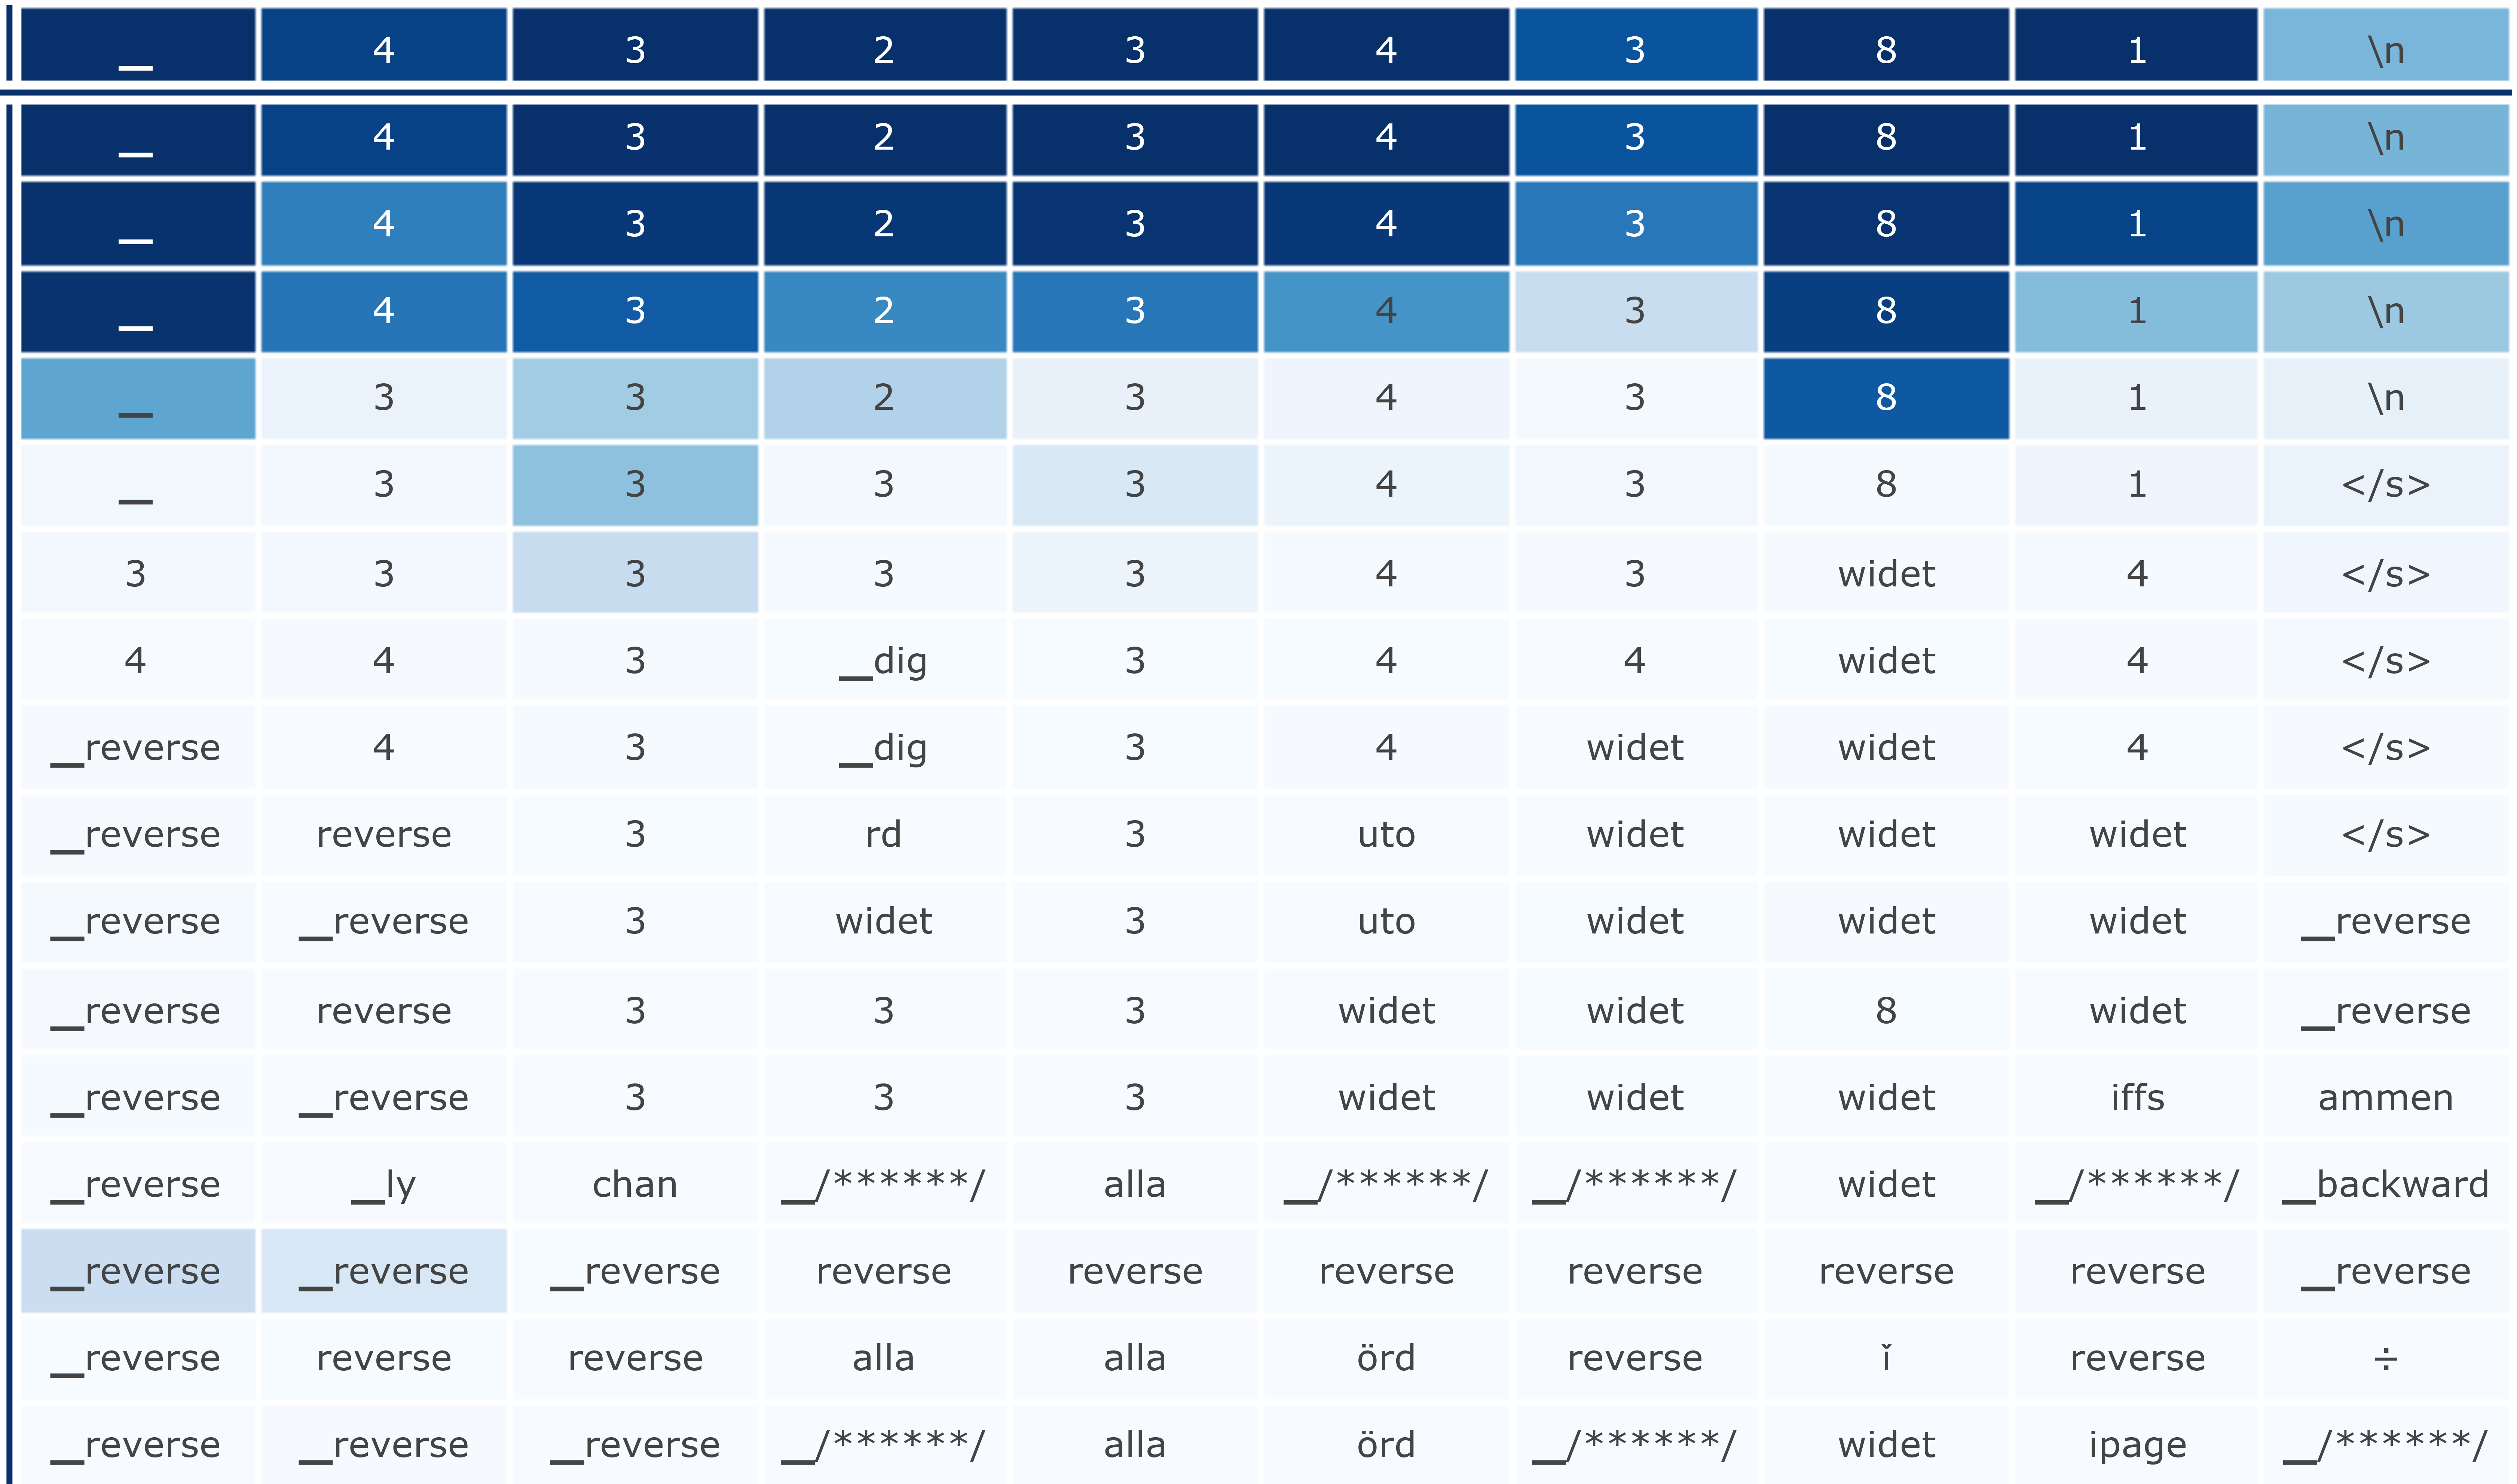
\includegraphics[width=0.95\textwidth]{exp_intravisto_4G_heatmap.png}}%
            %\end{overprint}%
            \begin{tikzpicture}
                \node (n) {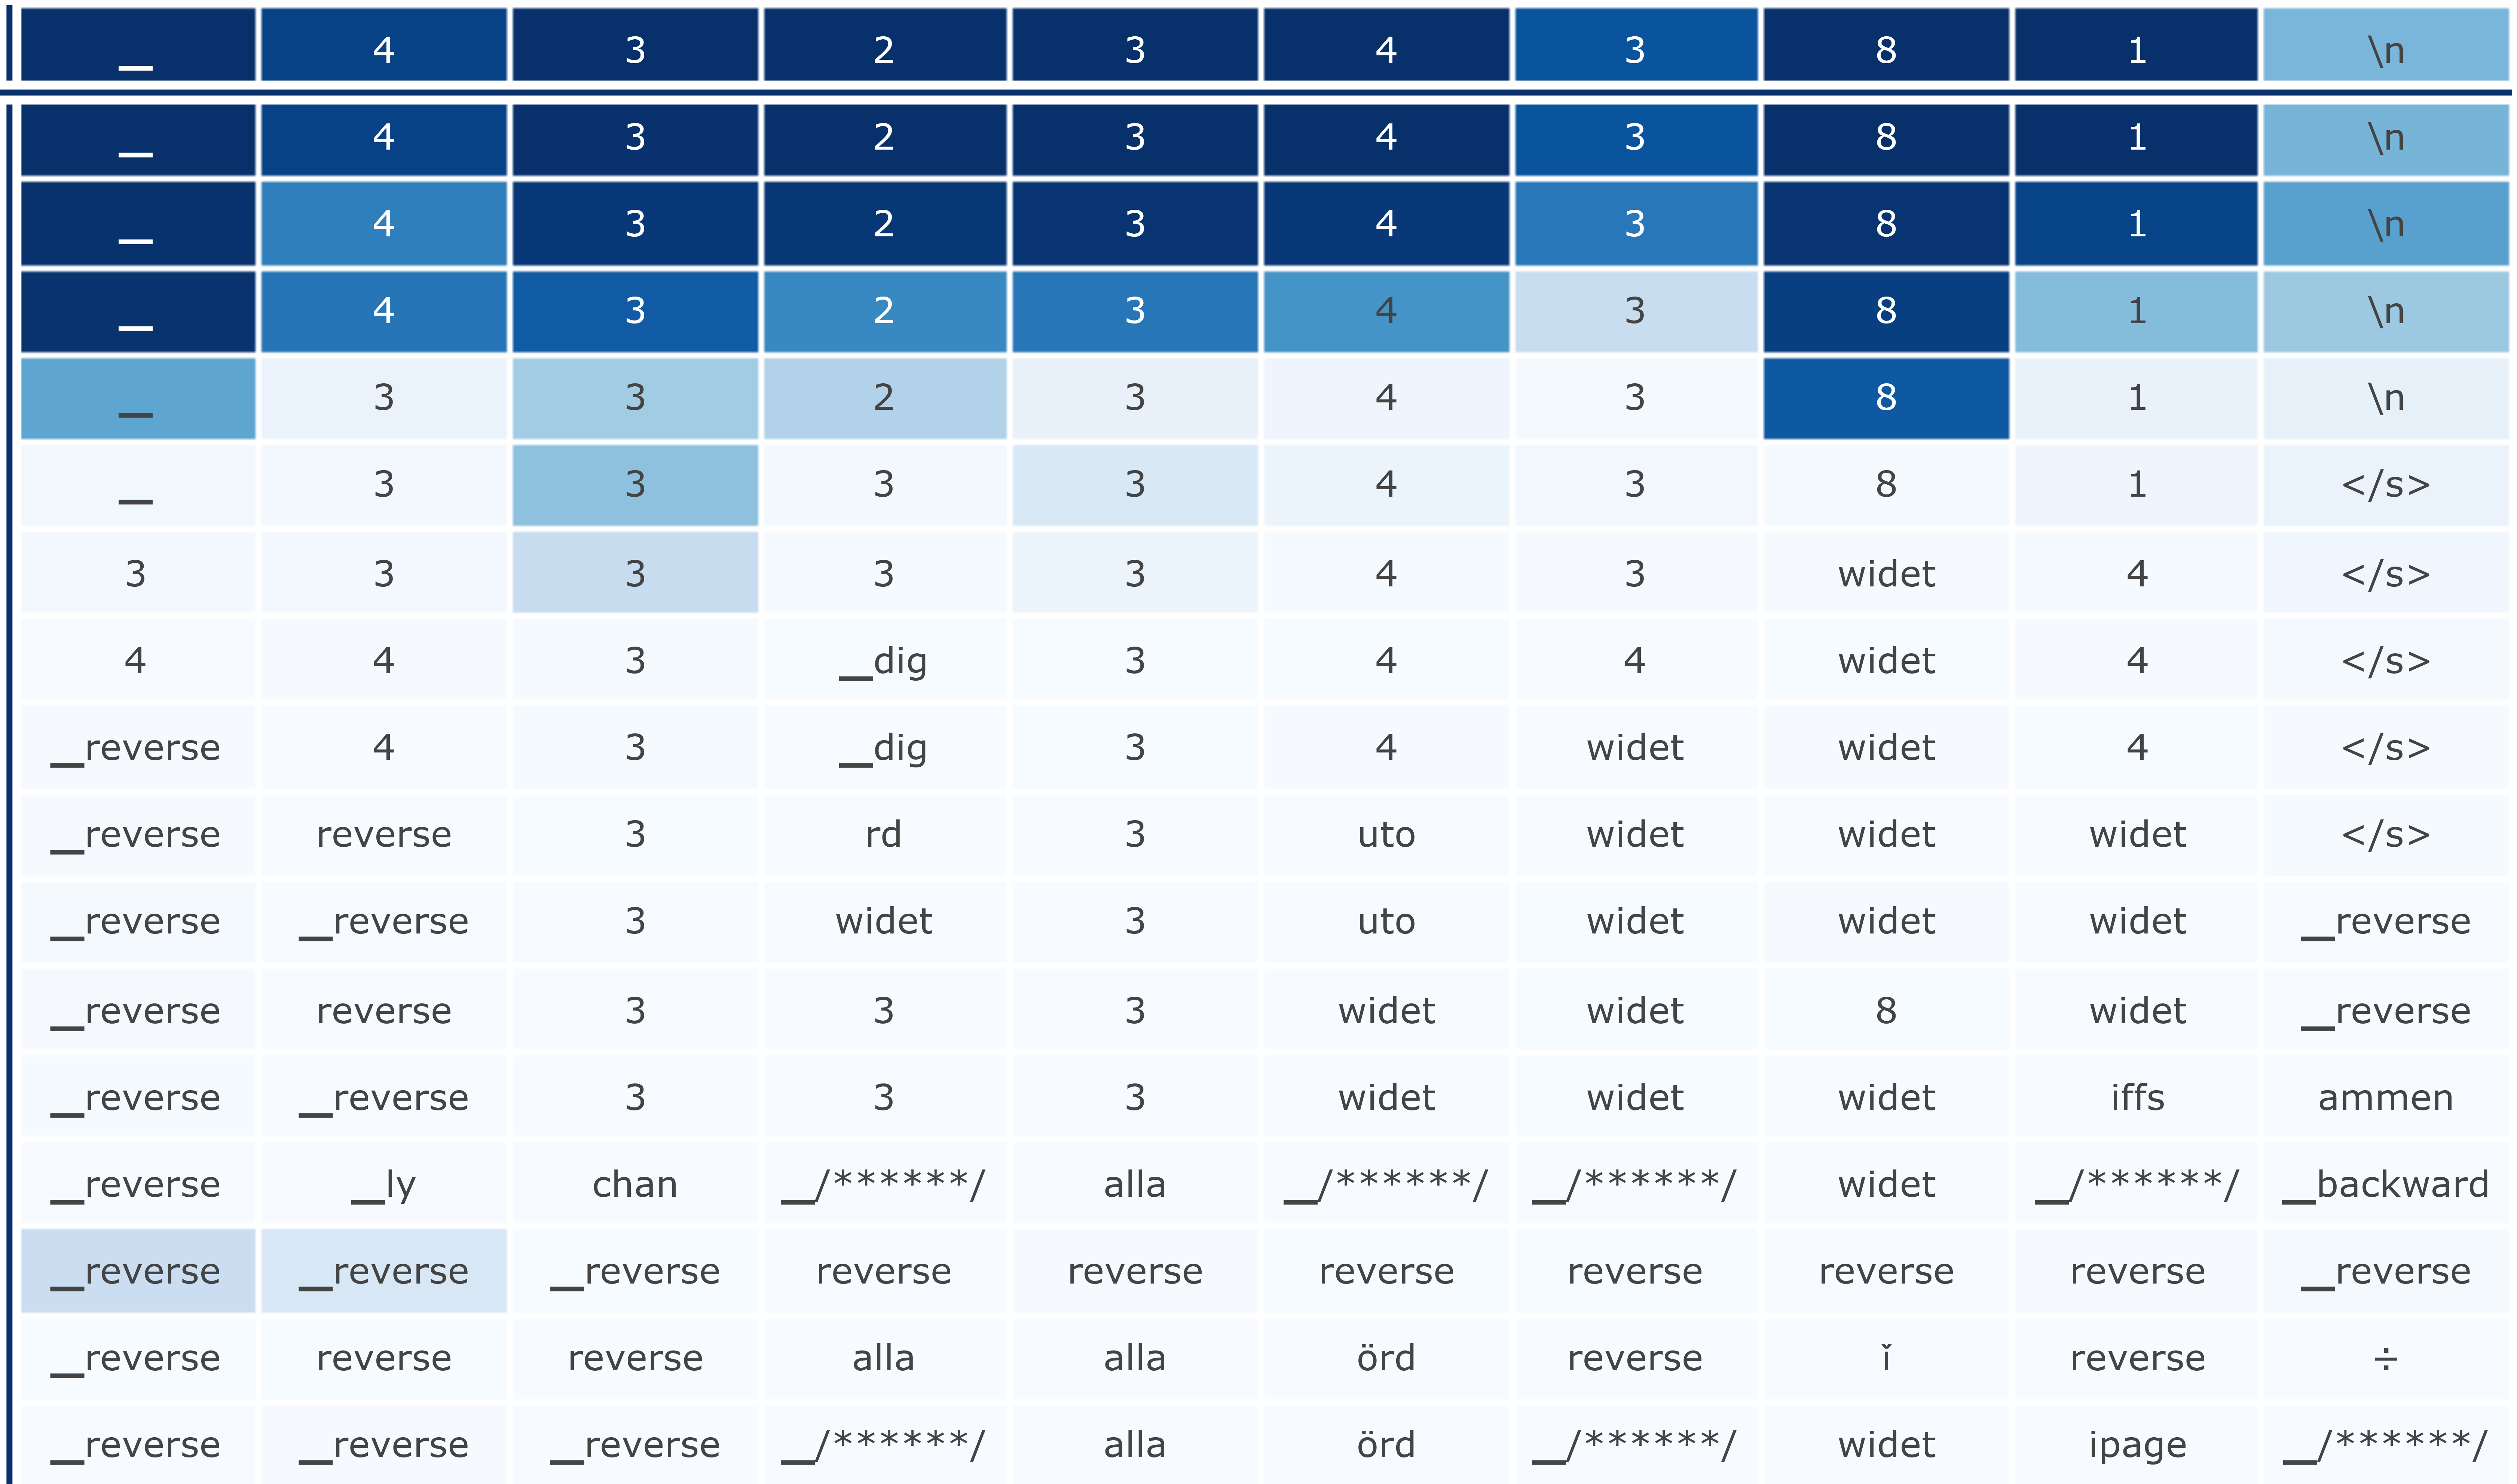
\includegraphics[width=0.95\textwidth]{exp_intravisto_4G_heatmap.png}};
                \draw[color=red,thick] (0.85,0.97) rectangle (1.75,2.56);
            \end{tikzpicture}
        \end{minipage}%
        \begin{minipage}{0.4\textwidth}
            \footnotesize
            \begin{itemize}[<+|visible@+->]
                \setlength\itemsep{0.2cm}
                %\item<1-1> By hovering over a cell, a pop-up with other possible decoded tokens (secondary representation) along with additional information appears.
                \item<1-1> The heatmap indicates a \emph{clear step} in the magnitude of token probabilities when passing from intermediate layers to final layers, which tends to happen earlier in layers as the next token becomes more obvious.
            \end{itemize}
        \end{minipage}
    \end{frame}

    \begin{frame}{Embedding Injection}
        \begin{minipage}{0.4\textwidth}
            \centering
            \begin{overprint}%
                \onslide<1-2>
                \overimage[0.7cm]{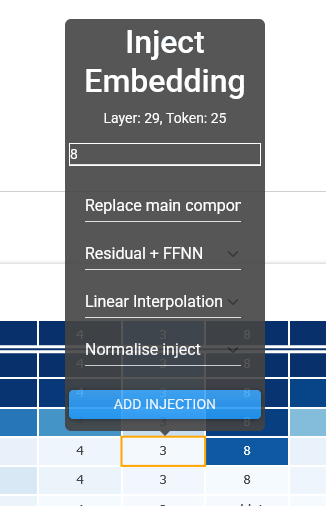
\includegraphics[width=0.65\textwidth]{pres_intravisto-injection.png}}%
            \end{overprint}%
        \end{minipage}%
        \begin{minipage}{0.6\textwidth}
            \footnotesize
            \begin{itemize}[<+|visible@+->]
                \setlength\itemsep{0.5cm}
                \item<1-1> Injections are performed by clicking on a cell in the heatmap or Sankey diagram and substitute hidden states with custom embedding representations, forcing the model to adjust its behavior based on the injected information.
                \item<2-2> We inject the correct digit ($8$) into the residual stream in order to sway the generative process of the model into returning the wanted result. 
            \end{itemize}
        \end{minipage}
    \end{frame}
    
    \begin{frame}[empty]{}
        \vspace*{-0.15cm}
        \only<1-2>{
            \begin{tikzpicture}
                \hspace*{-0.4cm}%
                \only<1>{\node[inner sep=0] (img) {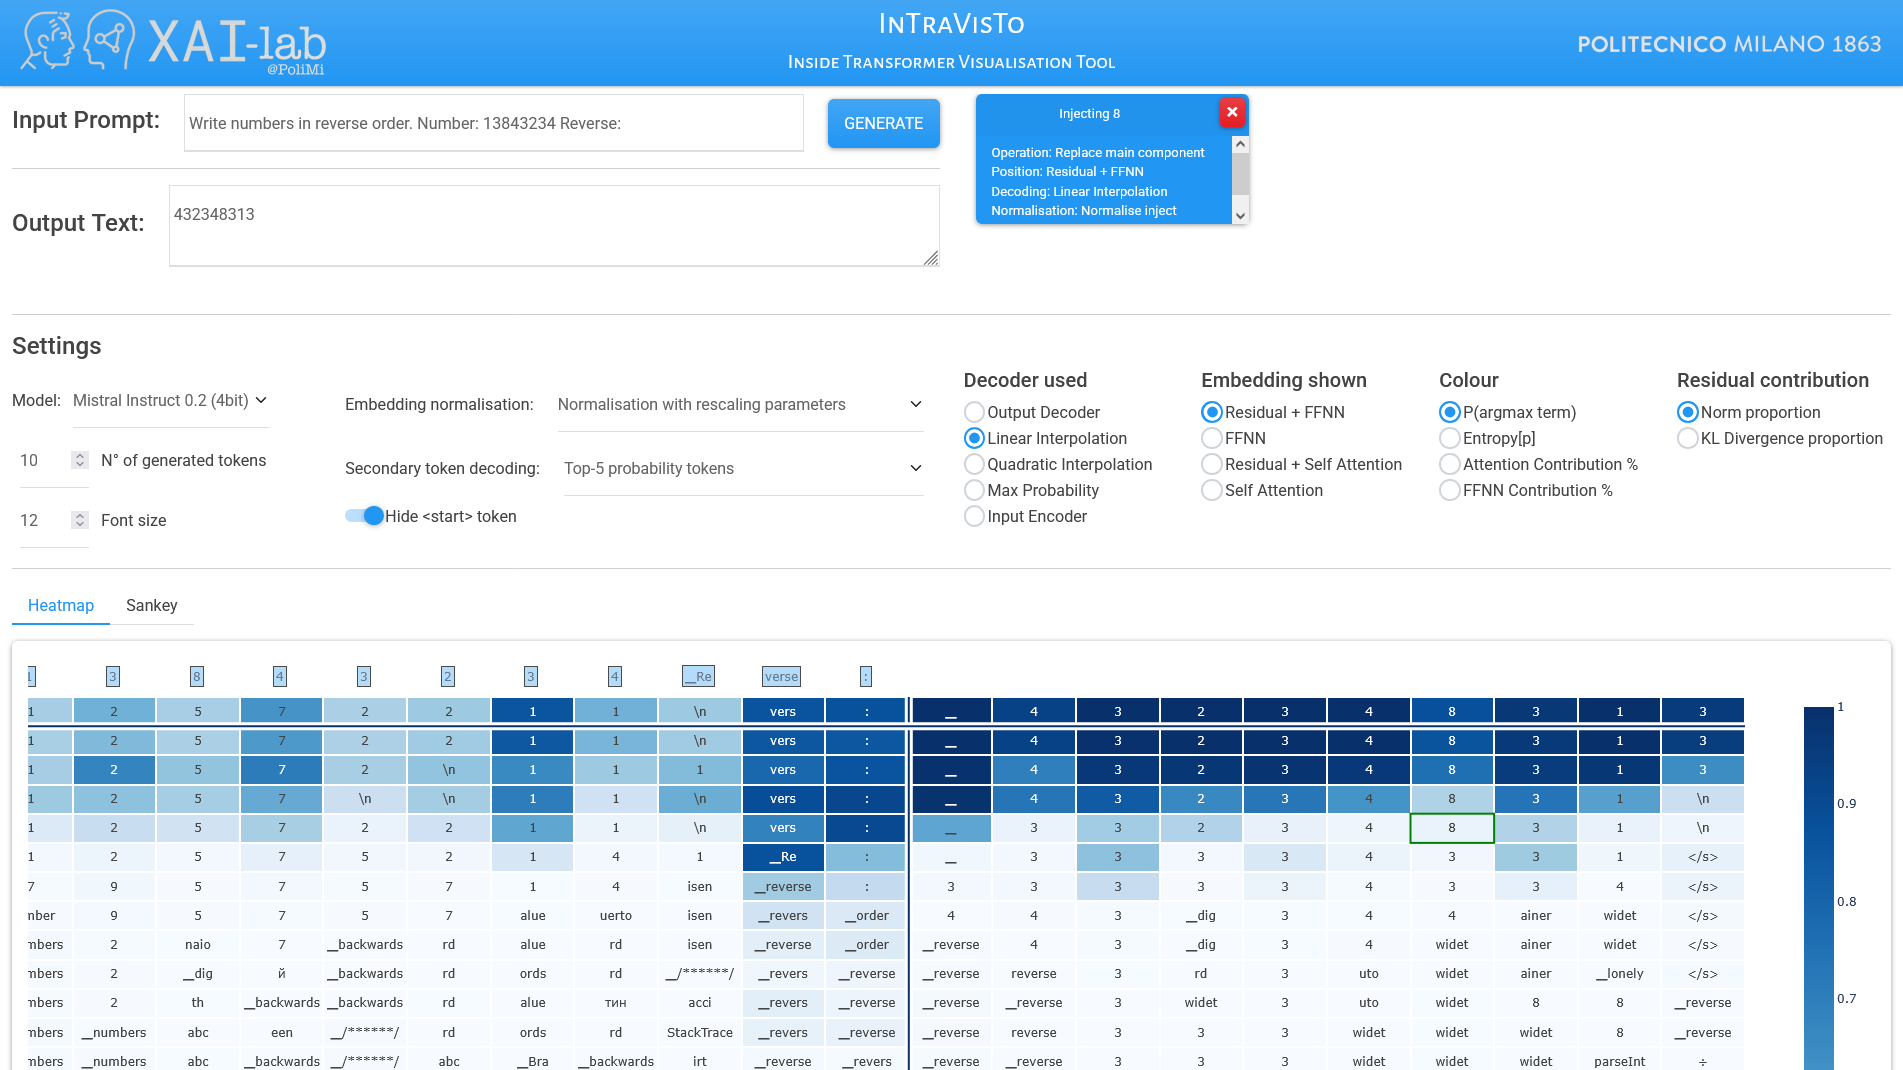
\includegraphics[width=\paperwidth]{pres_intravisto-injection-card.png}};}%
                \only<1>{\draw[color=red,thick] (0.13,2.55) rectangle (2.58,3.75);}
                \only<2>{\node[inner sep=0] (img) {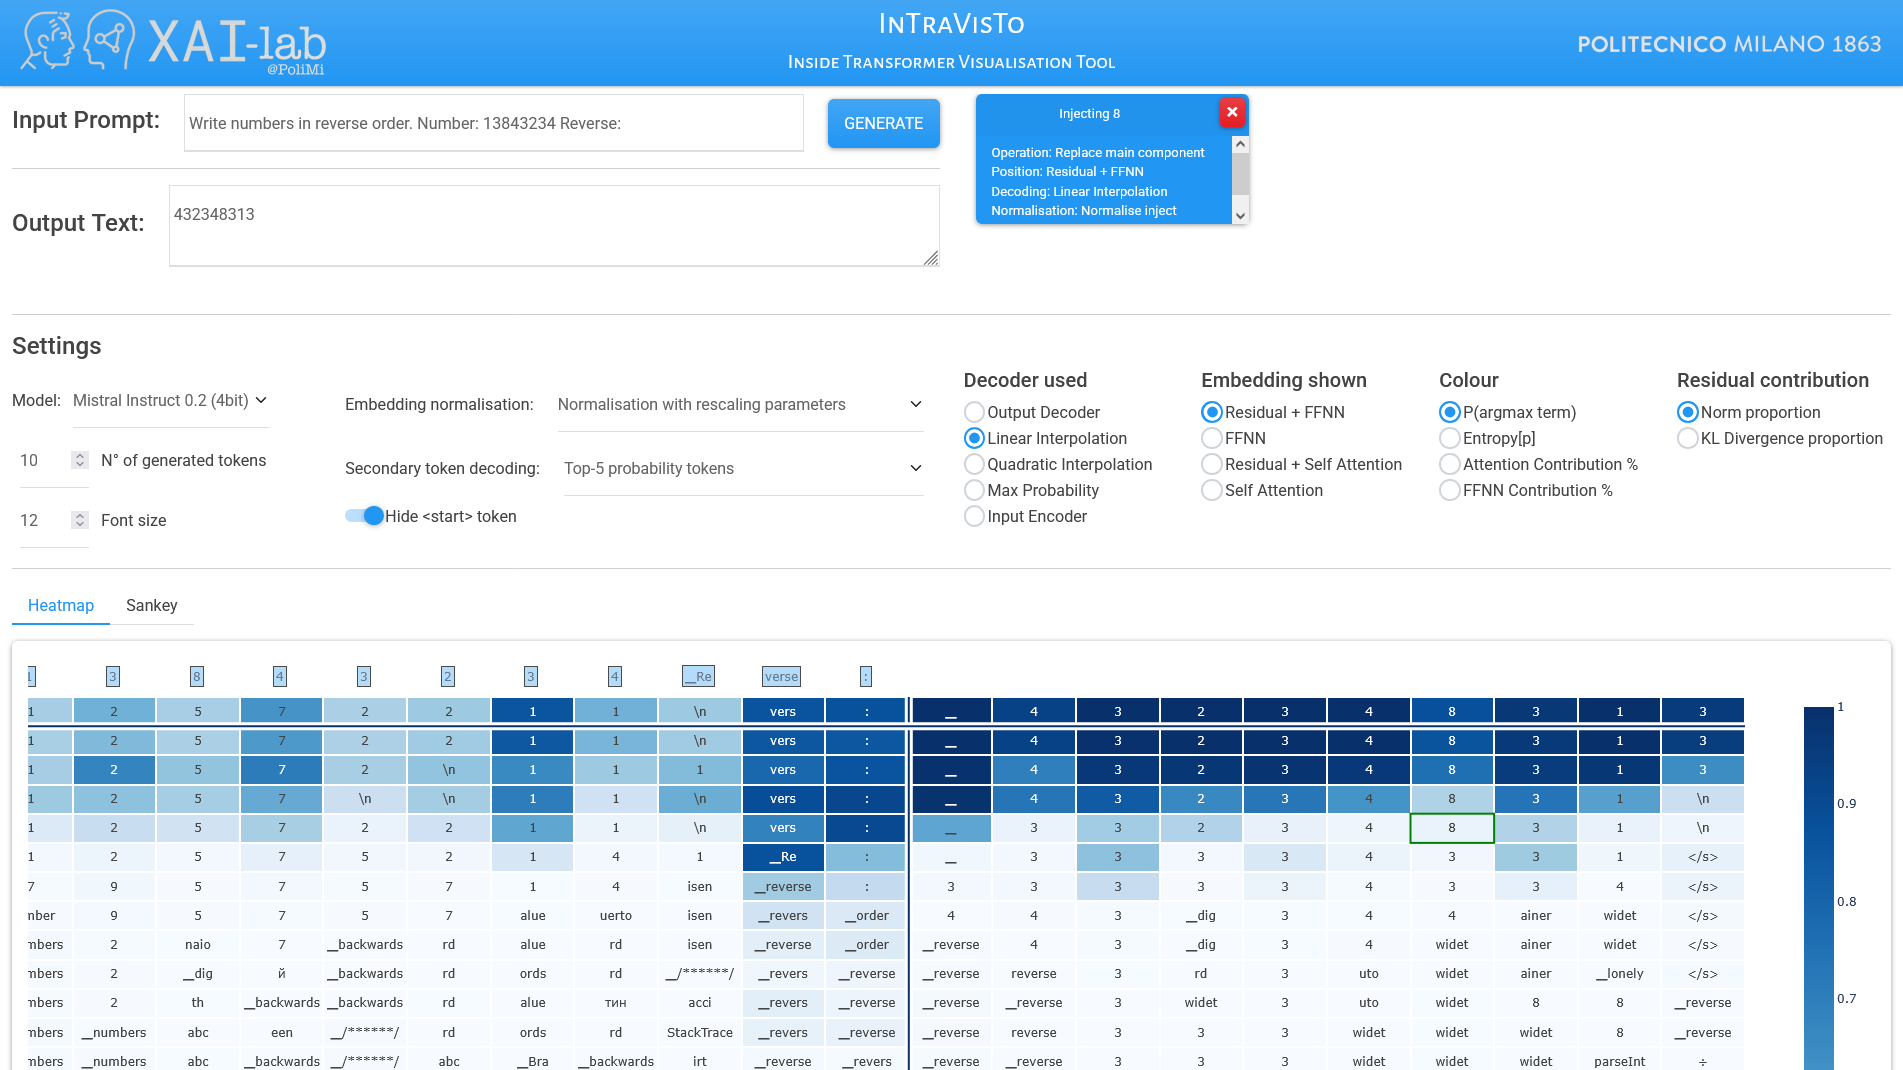
\includegraphics[width=\paperwidth]{pres_intravisto-injection-card.png}};}%
                \only<2>{\draw[color=red,thick] (-7.98,2.2) rectangle (-0.04,3.75);}
            \end{tikzpicture}%
        }%
    \end{frame}

    \begin{frame}{Output After Injection}
        \begin{minipage}{0.6\textwidth}
            \centering
            \begin{overprint}%
                \onslide<1-2>
                \overimage{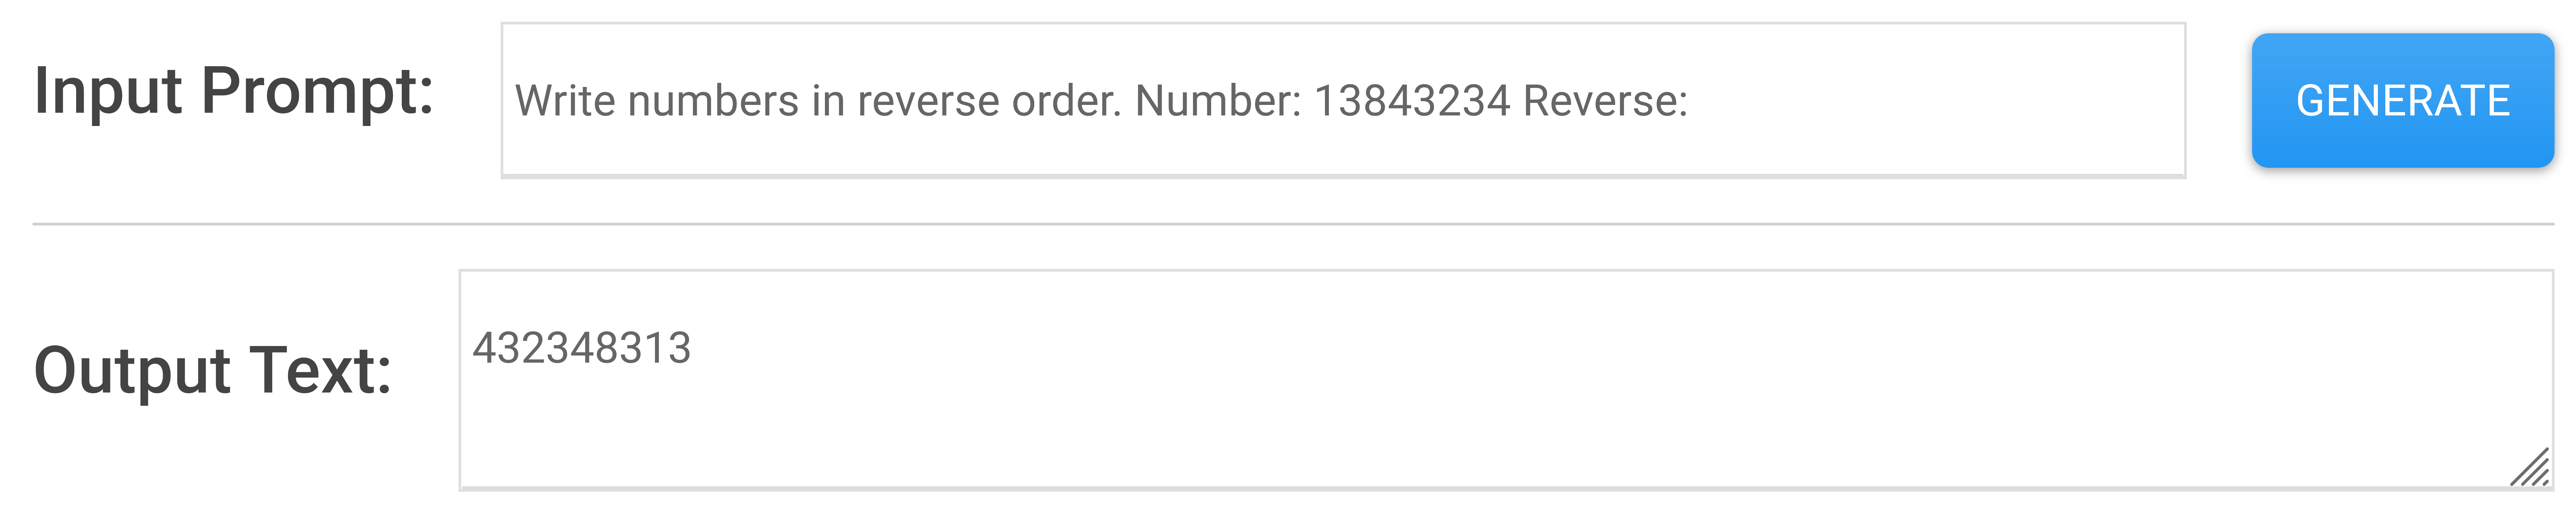
\includegraphics[width=0.95\textwidth]{pres_intravisto-example-injection-result.png}}%
            \end{overprint}%
        \end{minipage}%
        \begin{minipage}{0.4\textwidth}
            \footnotesize
            \begin{itemize}[<+|visible@+->]
                \setlength\itemsep{0.5cm}
                \item<1-1> After applying the injection, the model outputs the correct couple of digits ($83$) instead of the inverted $38$, thus the new output is \emph{``432348313''}.
                \item<2-2> However, the model generates an extra $3$ right at the end of the reversed number, instead of a newline character.
            \end{itemize}
        \end{minipage}
    \end{frame}

    \subsubsection{Flow Interface}

    \begin{frame}[empty]{}
        \vspace*{-0.15cm}
        \only<1-3>{
            \begin{tikzpicture}
                \hspace*{-0.4cm}%
                \only<1>{\node[inner sep=0] (img) {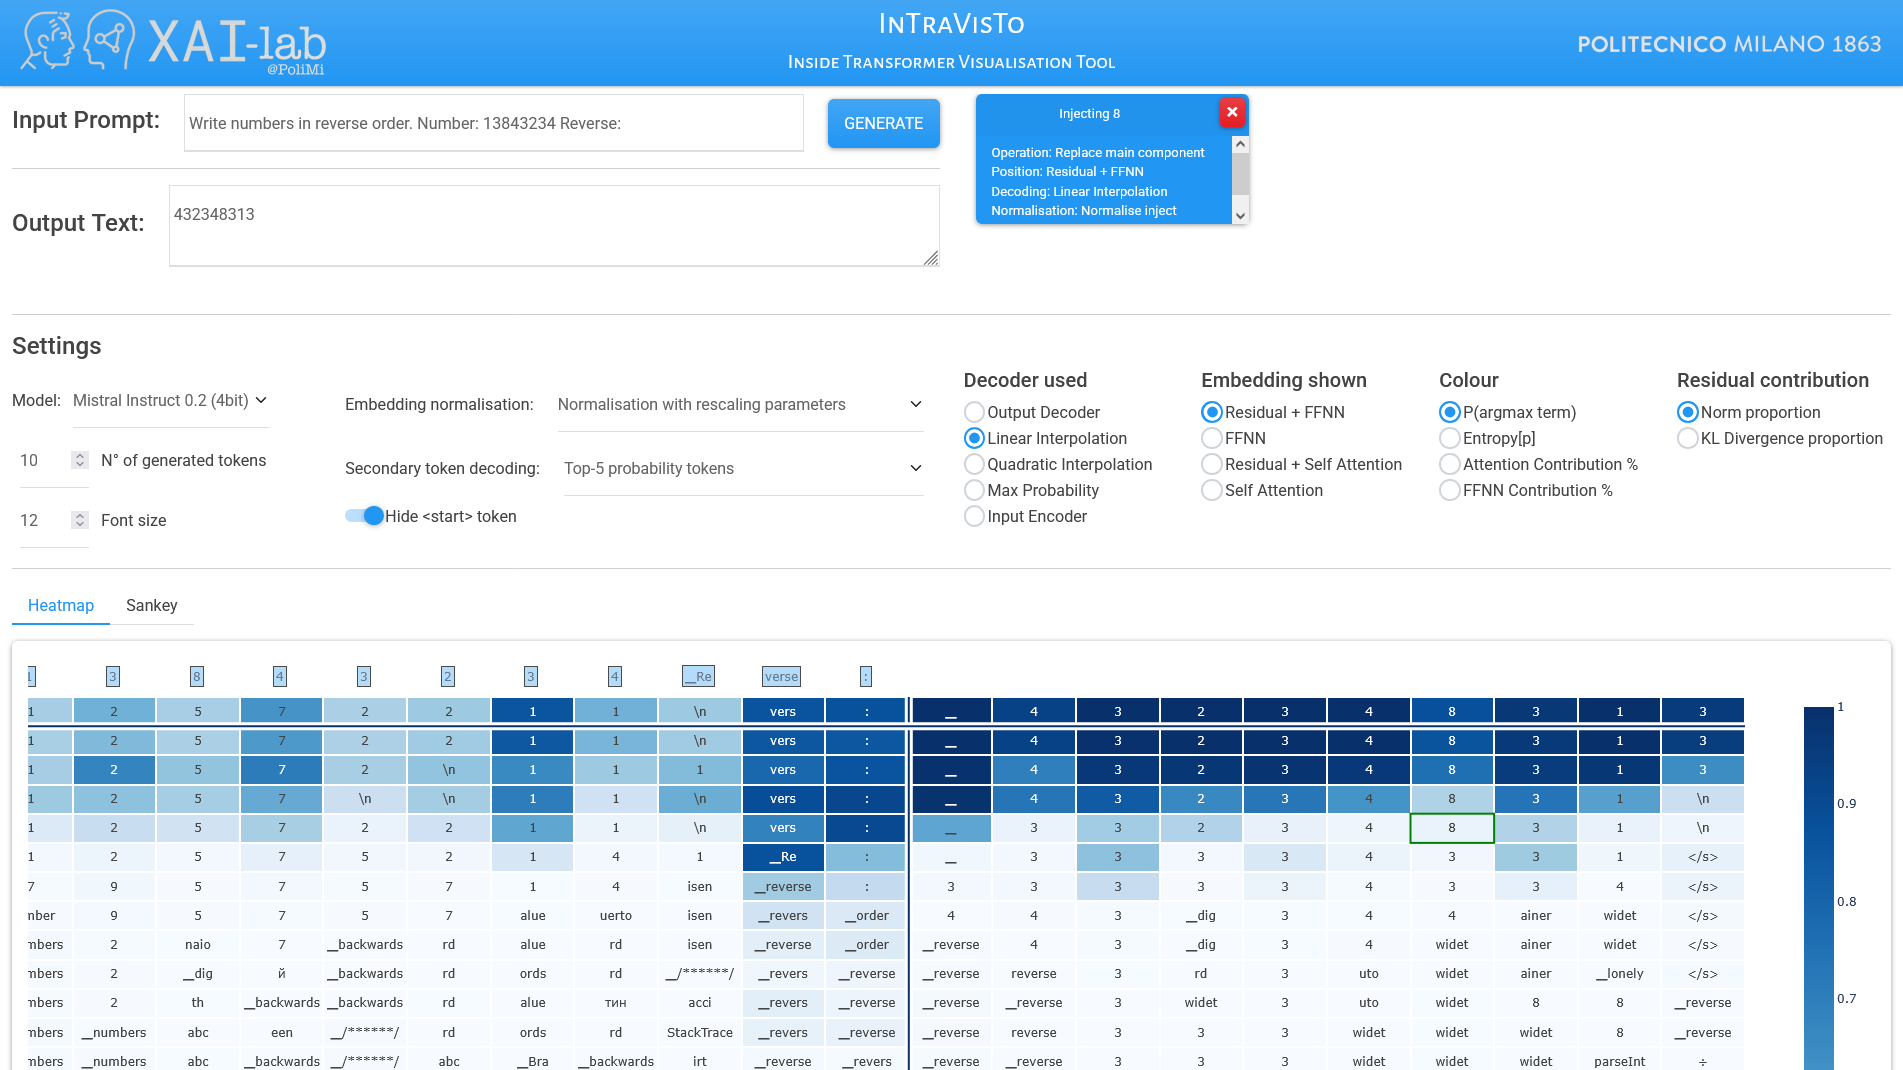
\includegraphics[width=\paperwidth]{pres_intravisto-injection-card.png}};}%
                \only<1>{\draw[color=red,thick] (-7.95,-0.8) rectangle (-6.25,-0.34);}
                \only<2>{\node[inner sep=0] (img) {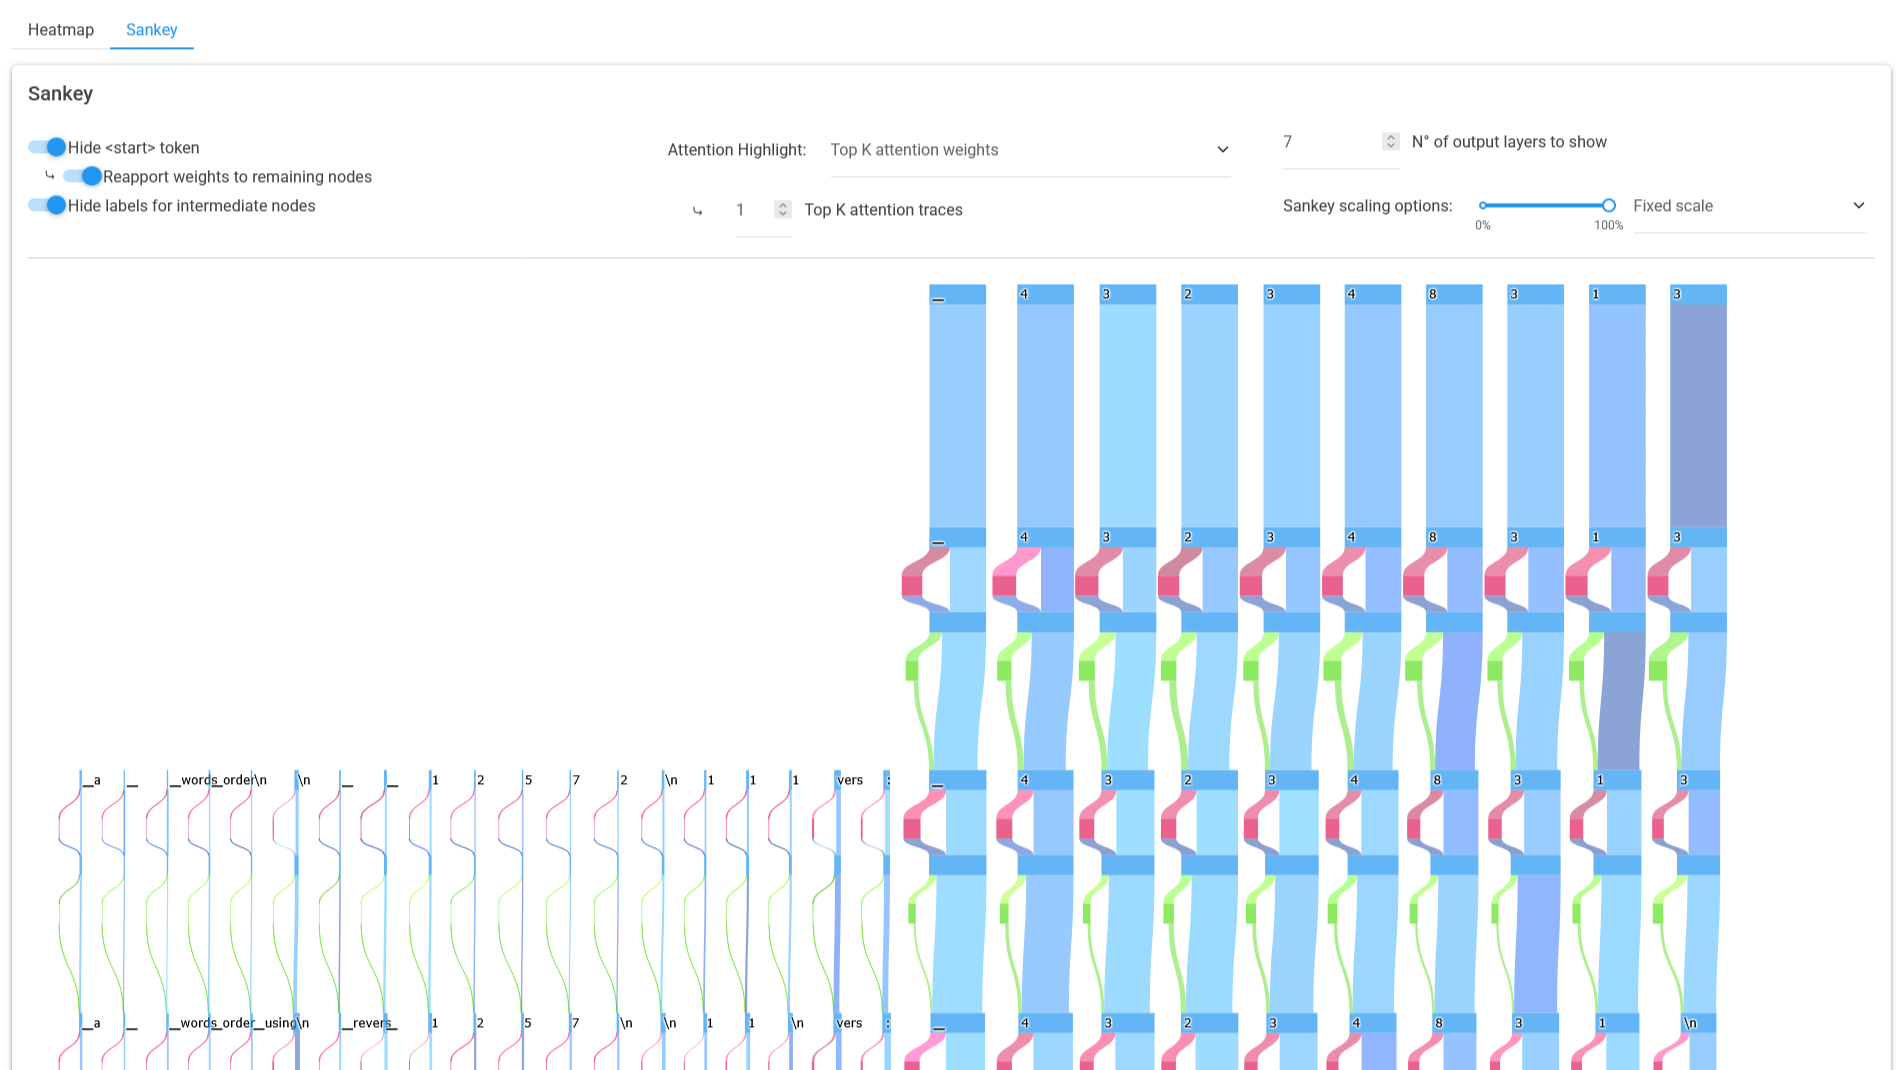
\includegraphics[width=\paperwidth]{pres_intravisto-sankey.png}};}%
                \only<3>{\node[inner sep=0] (img) {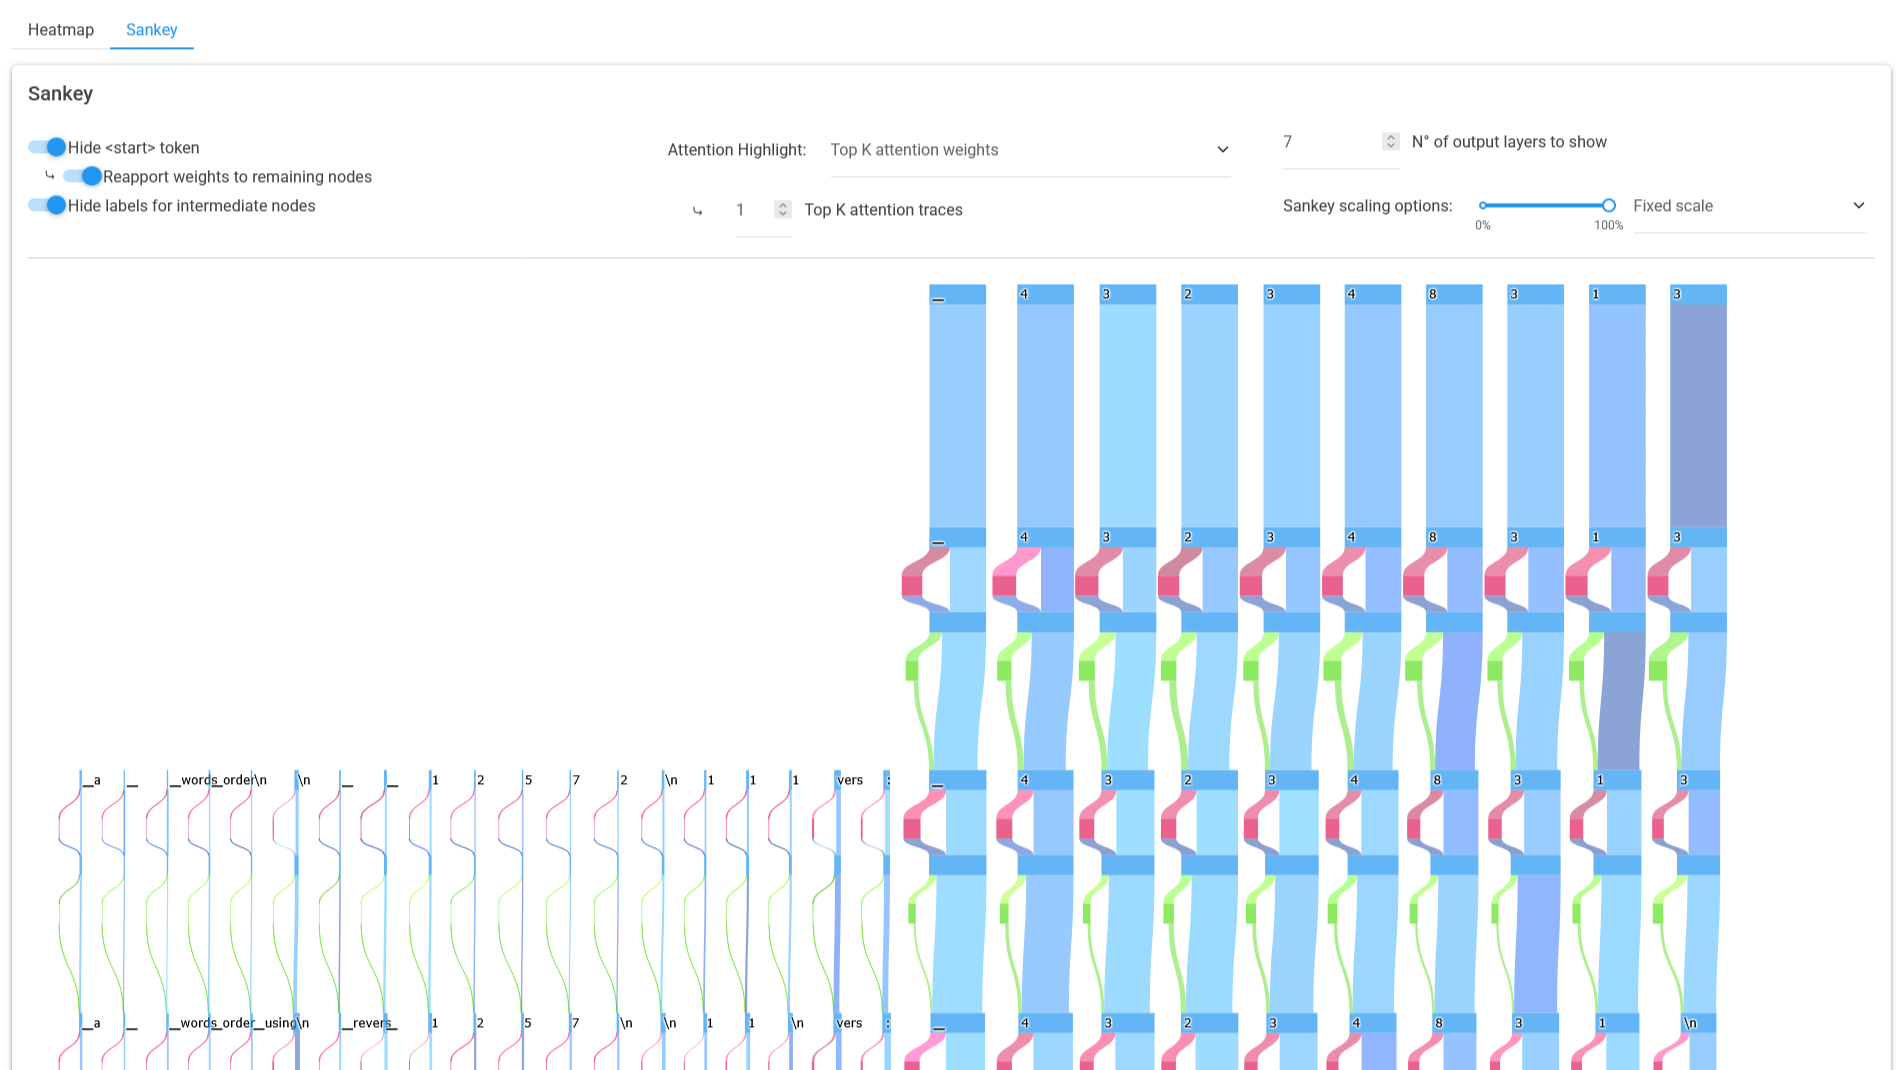
\includegraphics[width=\paperwidth]{pres_intravisto-sankey.png}};}%
                \only<3>{\draw[color=red,thick] (-0.46,-4.35) rectangle (6.6,2.25);}
            \end{tikzpicture}%
        }%
    \end{frame}

    \begin{frame}{Sankey Diagram}
        \begin{minipage}{0.55\textwidth}
            \begin{itemize}[<+|visible@+->]
                \setlength\itemsep{0.3cm}
                \item<1-1> Nodes in the diagram depict all hidden states contained in each layer visualizing the four main Transformer block vectors, while edges represent the amount of relevance carried by the residual stream, showing how components accumulate or disperse this flow.
                \item<2-2> The flow originates from the topmost layer of nodes, equally split between them, and is recursively computed considering the contributions of each encountered node.
            \end{itemize}
        \end{minipage}%
        \begin{minipage}{0.45\textwidth}
            \centering
            \begin{overprint}%
                \onslide<1>
                \overimage[0.6cm]{\hfill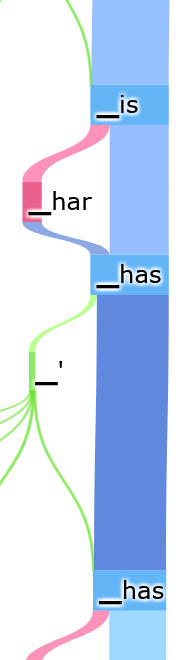
\includegraphics[width=0.25\textwidth]{pres_sankey.png}\hfill\includegraphics[width=0.53\textwidth]{pres_drw_transformer-no-in-out.pdf}\hfill}%
                \onslide<2>
                \overimage[0.7cm]{%
                \begin{tikzpicture}%
                    \node[inner sep=0] (img) {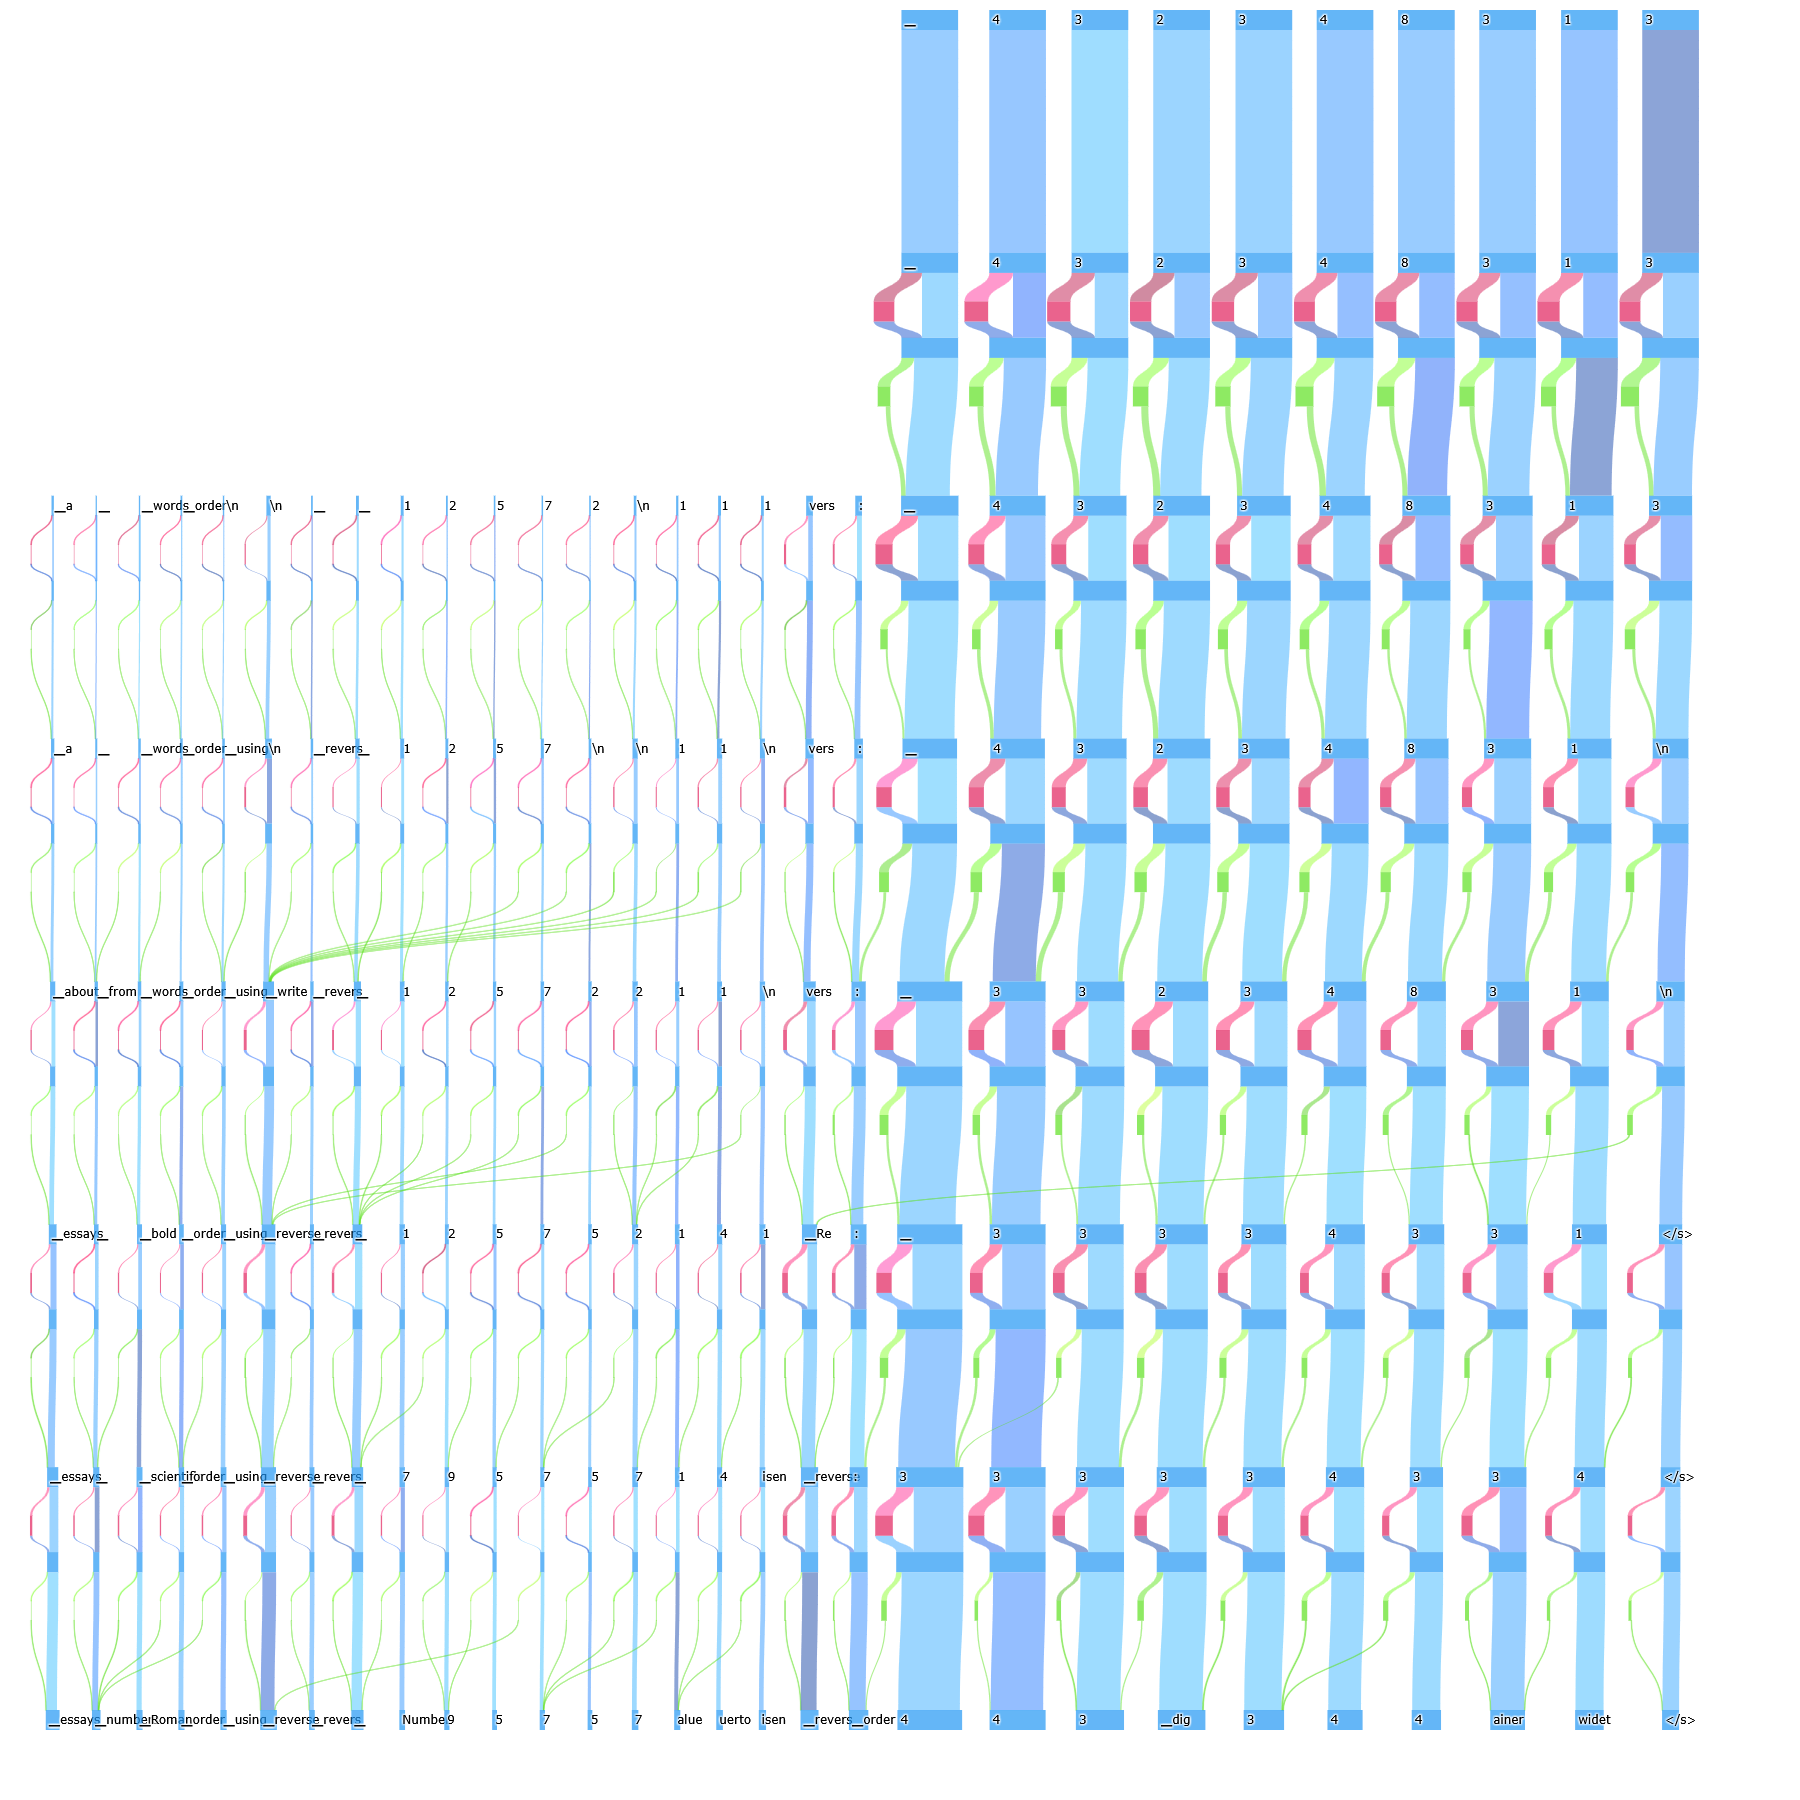
\includegraphics[width=0.9\textwidth]{pres_sankey-complete.png}};%
                    \node (ref) at (-4.5,-3.2) { };%
                    \node at (-2.8,2.3) {
                        \scalebox{0.32}{\parbox{\textwidth}_{\textit{ffnn}}^{(\ell,j)} \cdot \textit{flow}_{x}^{(\ell,j)} \\[2pt]
                                &\textit{flow}_{x'}^{(\ell,j)} &&= \textit{flow}_{\textit{ffnn}}^{(\ell,j)} + (1 - {\%}_{\textit{ffnn}}^{(\ell,j)})\textit{flow}_{\textit{x}}^{(\ell,j)} = \textit{flow}_{\textit{x}}^{(\ell,j)} \\[2pt]
                                &\textit{flow}_{\textit{att}}^{(\ell,j)} &&= {\%}_{\textit{att}}^{(\ell,j)} \cdot \textit{flow}_{x'}^{(\ell,j)} = {\%}_{\textit{att}}^{(\ell,j)} \cdot \textit{flow}_{x}^{(\ell,j)} \\[2pt]
                                &\textit{flow}_{x}^{(\ell-1,j)} &&= \sum_{i\in\{j,\ldots,k\}}{\overline{\textit{attend}{\,}}^{(\ell,i)}\bigl[j\bigr]}\cdot\textit{flow}_{\textit{att}}^{(\ell,i)} + ( 1 - {\%}_{\textit{att}}^{(\ell,j)}) \textit{flow}_{\textit{x'}}^{(\ell,j)} \\
                                    &\quad &&= \biggl(\Bigl(\sum_{i\in\{j,\ldots,k\}}\overline{\textit{attend}{\,}}^{(\ell,i)}\bigl[j\bigr] - 1\Bigr){\%}_{\textit{att}}^{(\ell,j)} + 1\biggr) \textit{flow}_{\textit{x}}^{(\ell,j)}
                            \end{alignedat}
                            \right.
                        \end{equation*}}}%
                    };
                \end{tikzpicture}%
                }%
            \end{overprint}%
        \end{minipage}
    \end{frame}

    \begin{frame}{Component Ablation}
        \begin{minipage}{0.59\textwidth}
            \begin{itemize}[<+|visible@+->]
                \setlength\itemsep{0.5cm}
                \item<1-1> The extra $3$ can be traced back to the feed-forward contribution of layer $31$, since until that point the decoded residual reads ``\textbackslash{}n''.
                \item<2-2> We perform an \emph{ablation} by clicking on the node and selecting the option to remove its contribution from the model computation.
            \end{itemize}
        \end{minipage}%
        \begin{minipage}{0.41\textwidth}
            \centering
            \begin{overprint}%
                \onslide<1>
                \overimage[0.7cm]{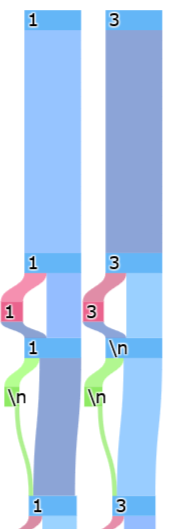
\includegraphics[width=0.31\textwidth]{pres_intravisto-example-injection.png}}%
                \onslide<2>
                \overimage[0.7cm]{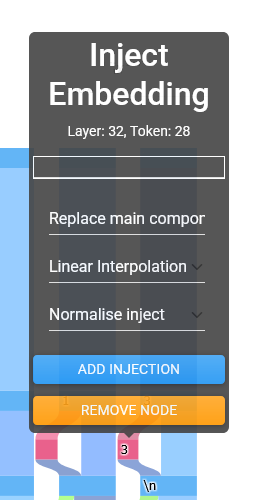
\includegraphics[width=0.5\textwidth]{pres_ablation-tooltip-example.png}}%
            \end{overprint}%
        \end{minipage}
    \end{frame}

    \begin{frame}{Output After Ablation}
        \begin{minipage}{0.6\textwidth}
            \centering
            \begin{overprint}%
                \onslide<1>
                \overimage[0.5cm]{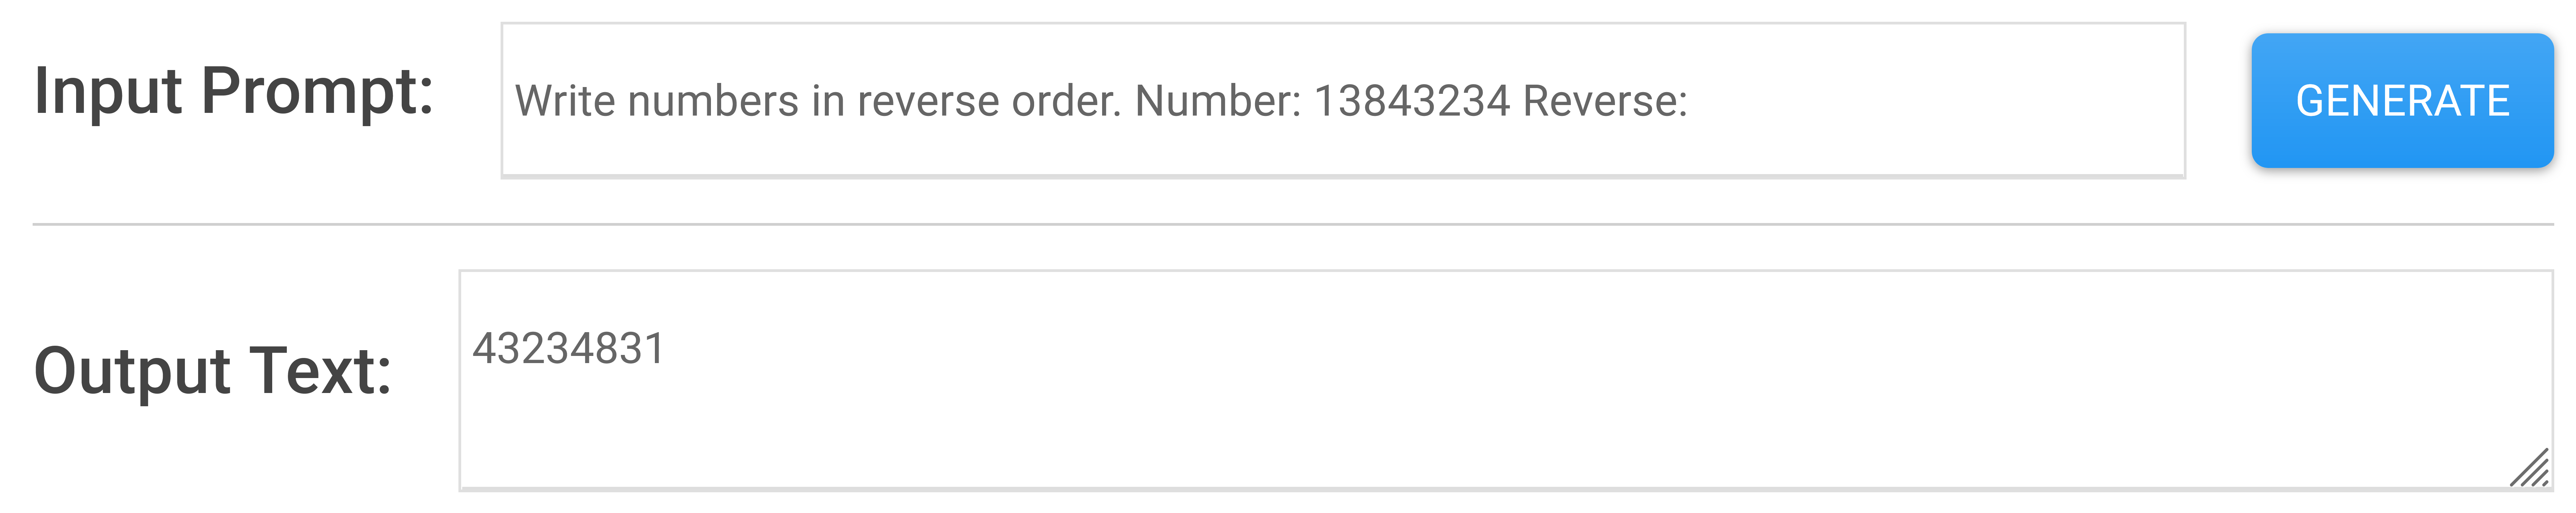
\includegraphics[width=0.95\textwidth]{pres_intravisto-example-ablation-result.png}}%
                \onslide<2>
                \overimage[0.5cm]{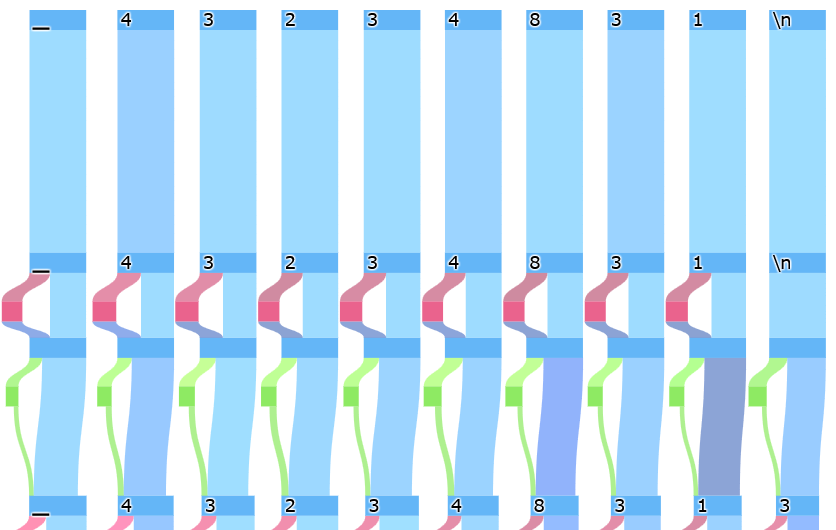
\includegraphics[width=0.9\textwidth]{pres_intravisto-example-ablation.png}}%
            \end{overprint}%
        \end{minipage}%
        \begin{minipage}{0.4\textwidth}
            \footnotesize
            \begin{itemize}[<+|visible@+->]
                \setlength\itemsep{0.5cm}
                \item<1-1> At this point, the model outputs \emph{``43234831''}, which is the correct result.
                \item<2-2> By removing the contribution of one specific feed-forward block, the model is able to avoid erroneously changing the content of its residual stream.
                The hidden state of the block is still decoded separately and can be inspected as usual.
            \end{itemize}
        \end{minipage}
    \end{frame}

    %\subsection{Other Examples}

    %\begin{frame}{Decimal Positions}
    %    \begin{minipage}{\textwidth}
    %        Models with dedicated tokens for each digit, when asked to perform arithmetic operations, happen to represent \emph{decimal positional information} along with digits of the result.
    %    \end{minipage}
    %    \begin{minipage}{\textwidth}
    %        \vspace{0.5cm}
    %        \centering
    %        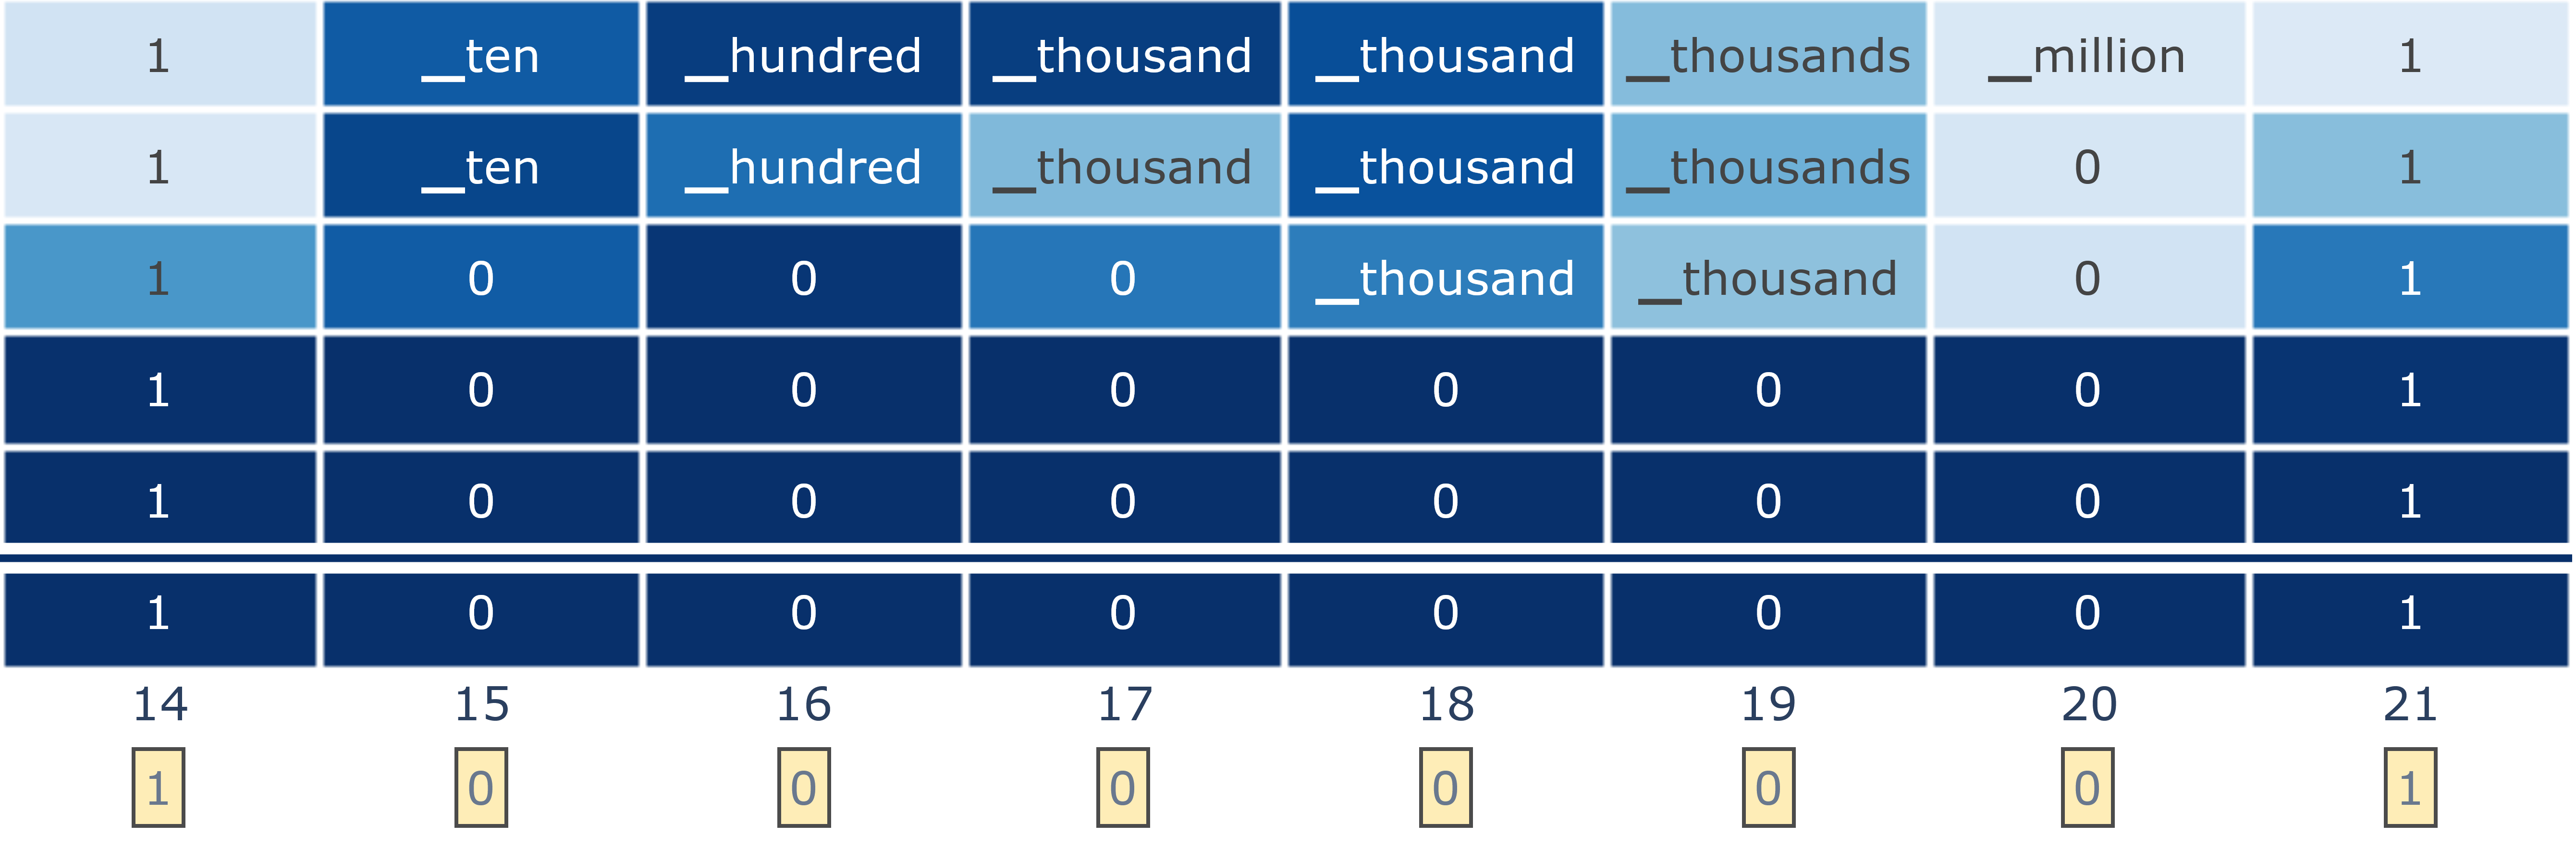
\includegraphics[width=0.8\textwidth]{exp_intravisto_4A_decimal.png}%
    %    \end{minipage}
    %\end{frame}

    %\begin{frame}{Alternative Representations}
    %    Other interesting representations of numbers can be noticed by directly analyzing single instances of numerical tokens and observing their alternative representations.
    %    \begin{minipage}{\textwidth}
    %        \vspace{0.5cm}
    %        \centering
    %        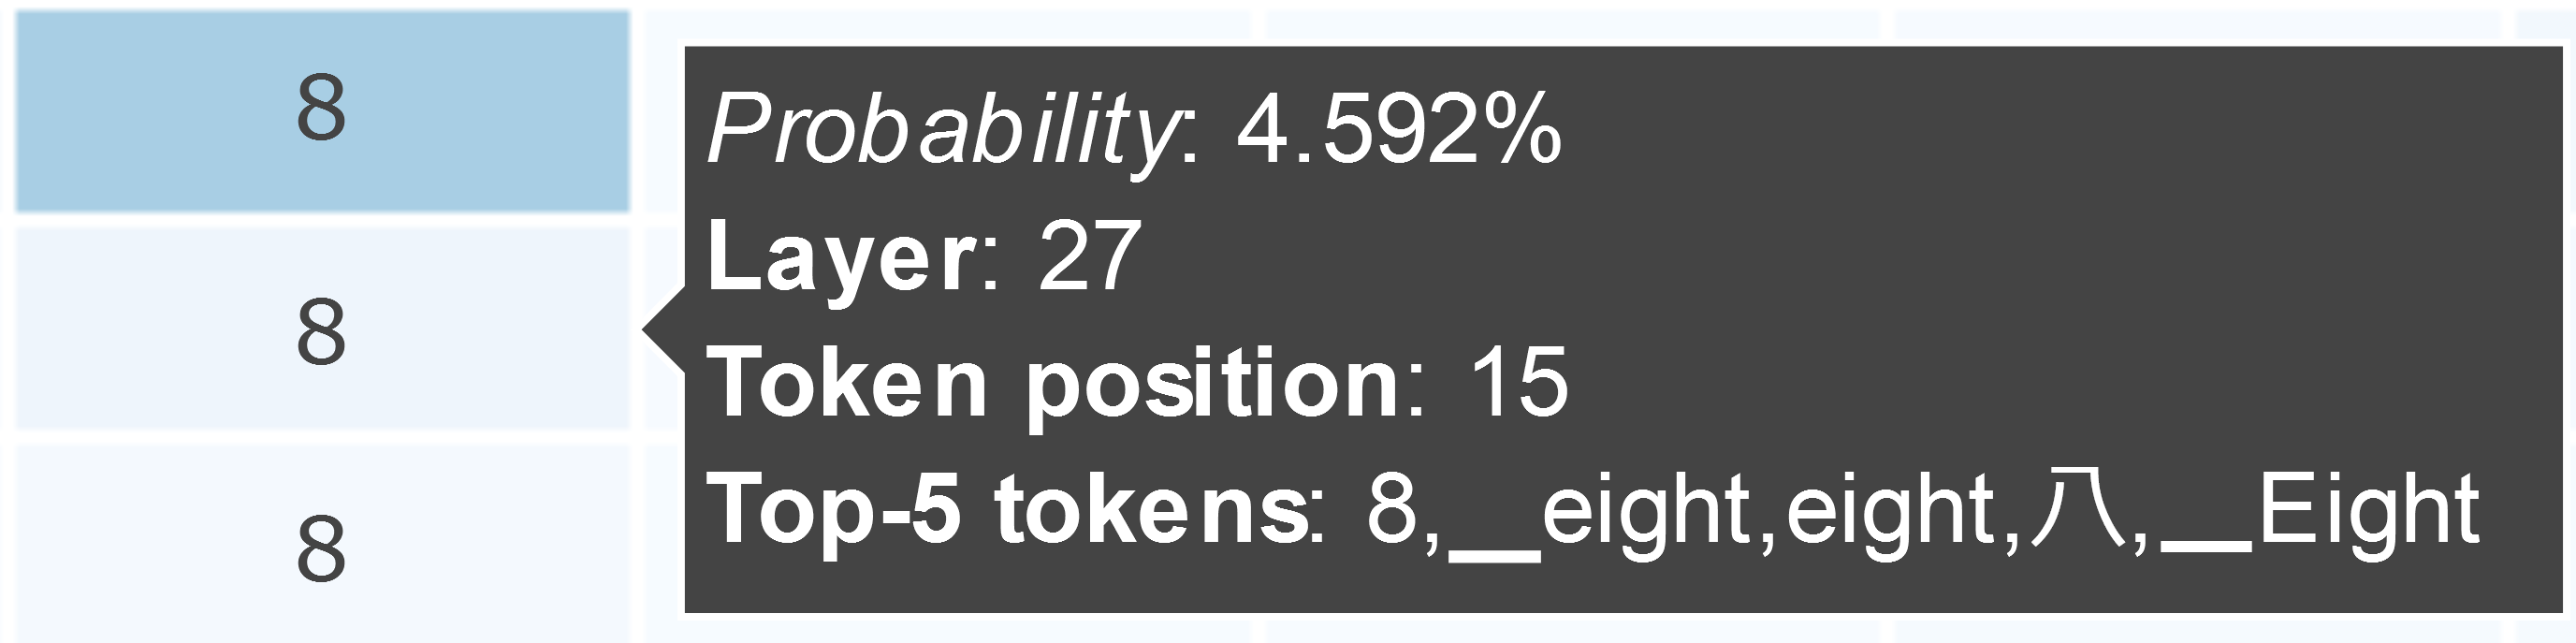
\includegraphics[width=0.5\textwidth]{exp_intravisto_4B_eight.png}%
    %        \hfill
    %        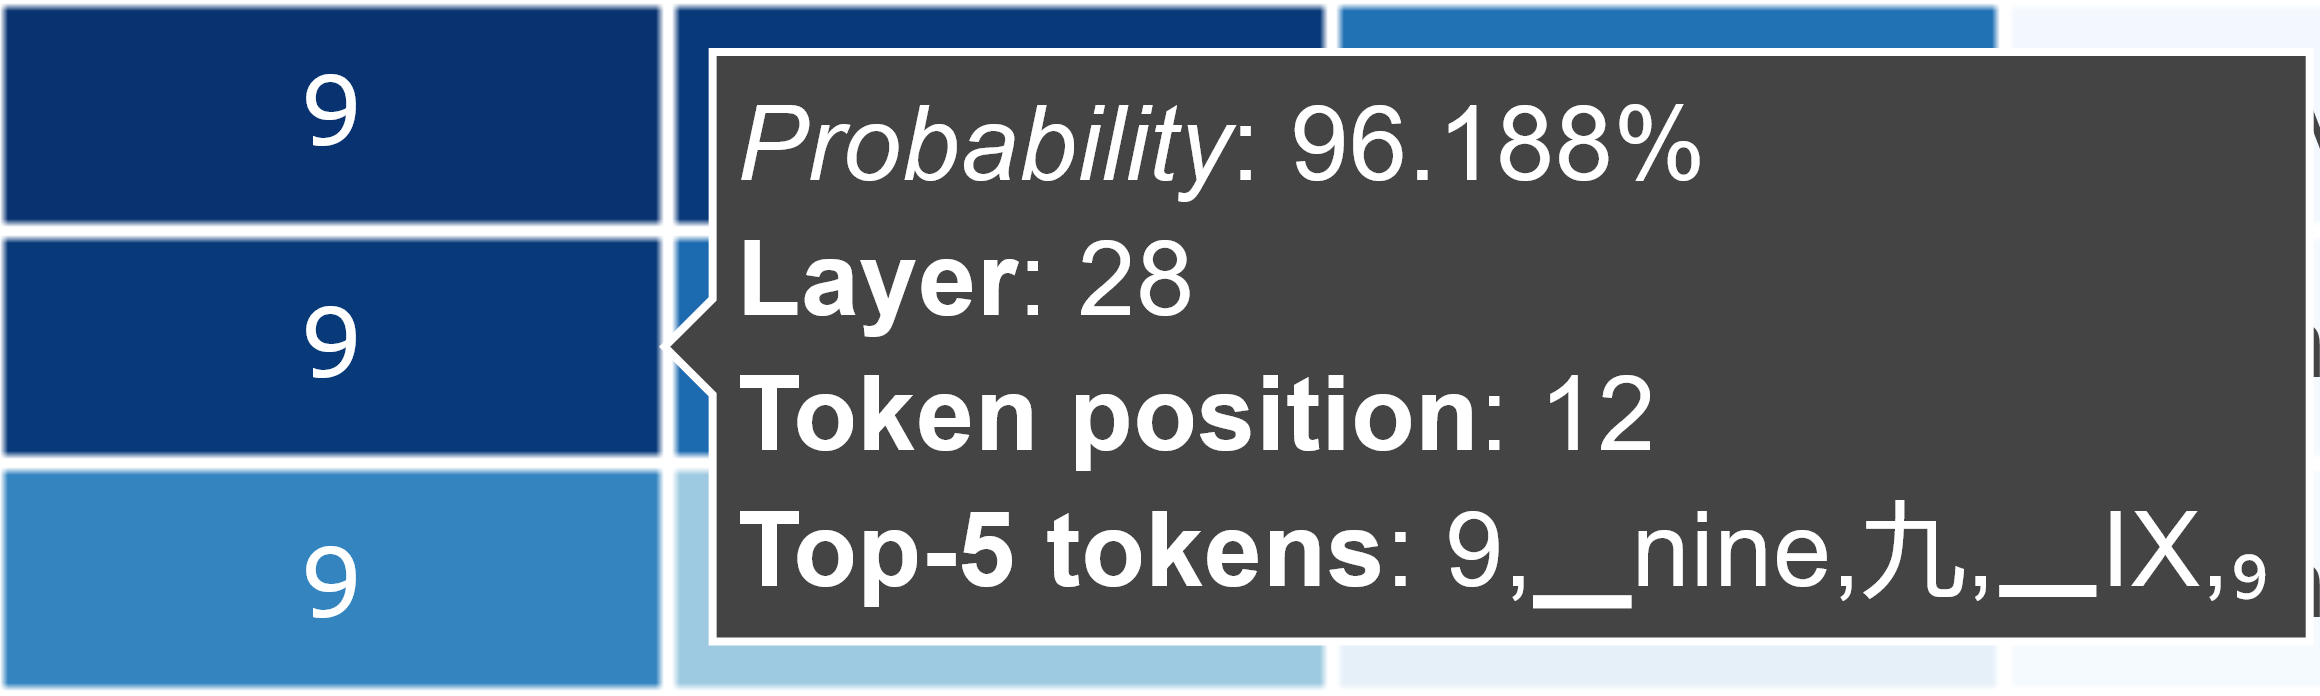
\includegraphics[width=0.4\textwidth]{exp_intravisto_4B_roman.png}%
    %    \end{minipage}
    %    \begin{minipage}{\textwidth}
    %        \vspace{0.25cm}
    %        \centering
    %        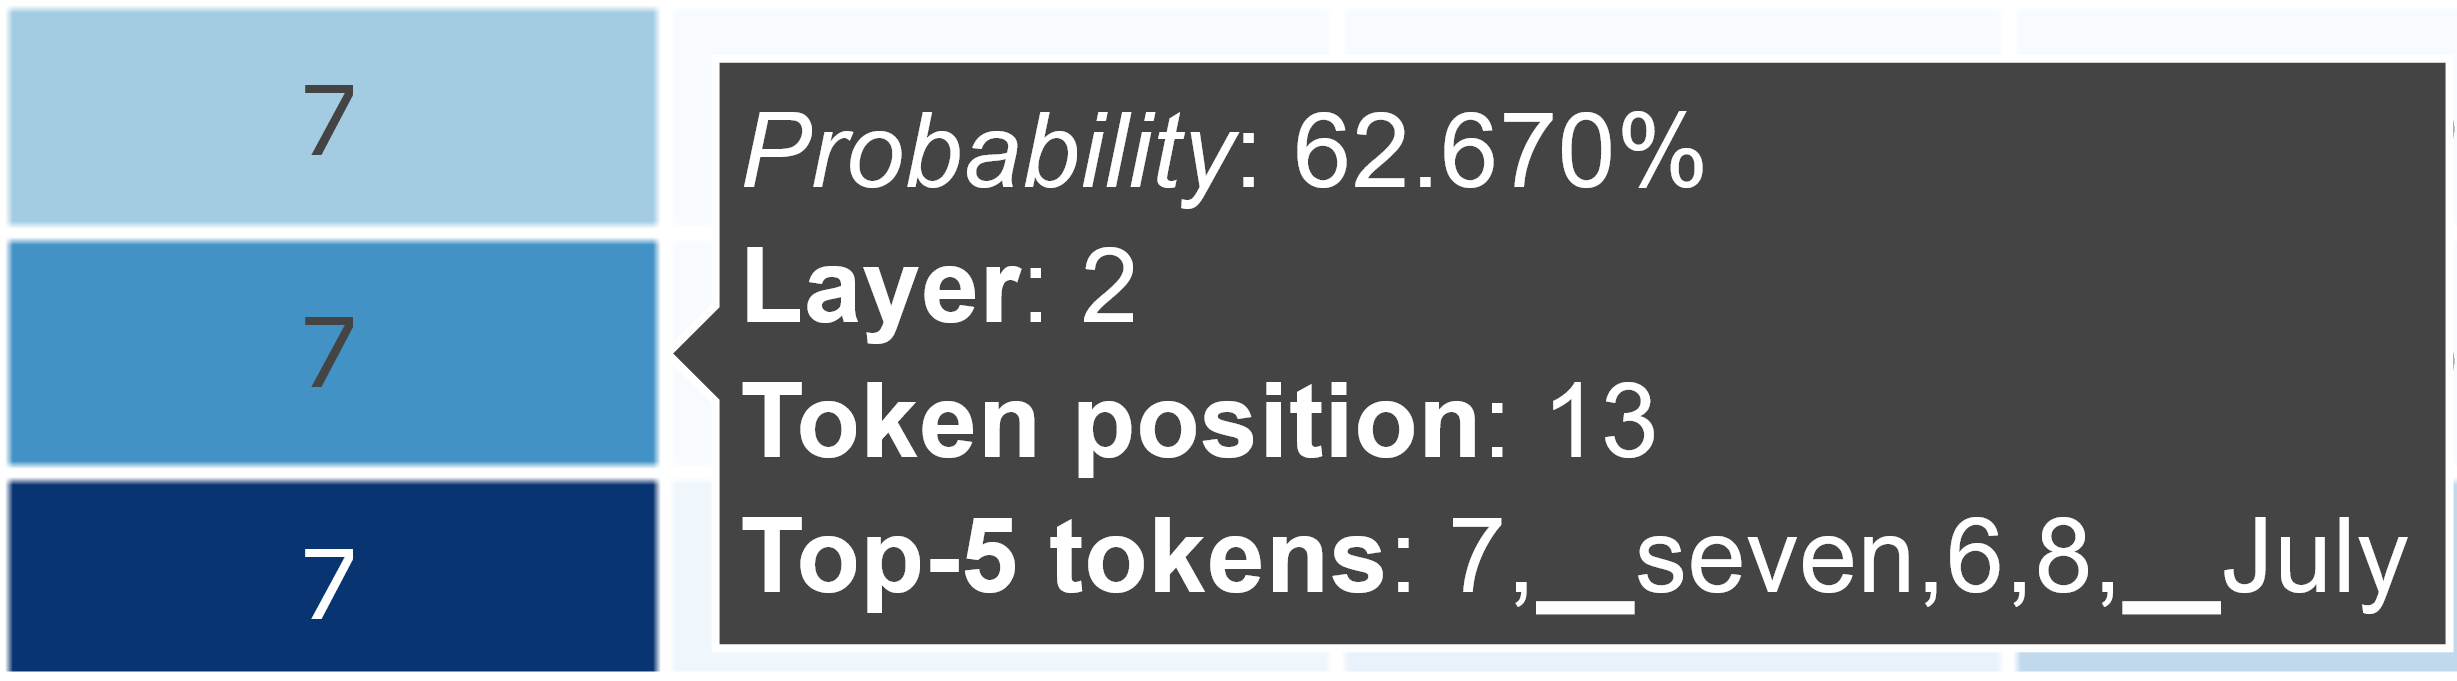
\includegraphics[width=0.45\textwidth]{exp_intravisto_4B_month.png}%
    %        \hfill
    %        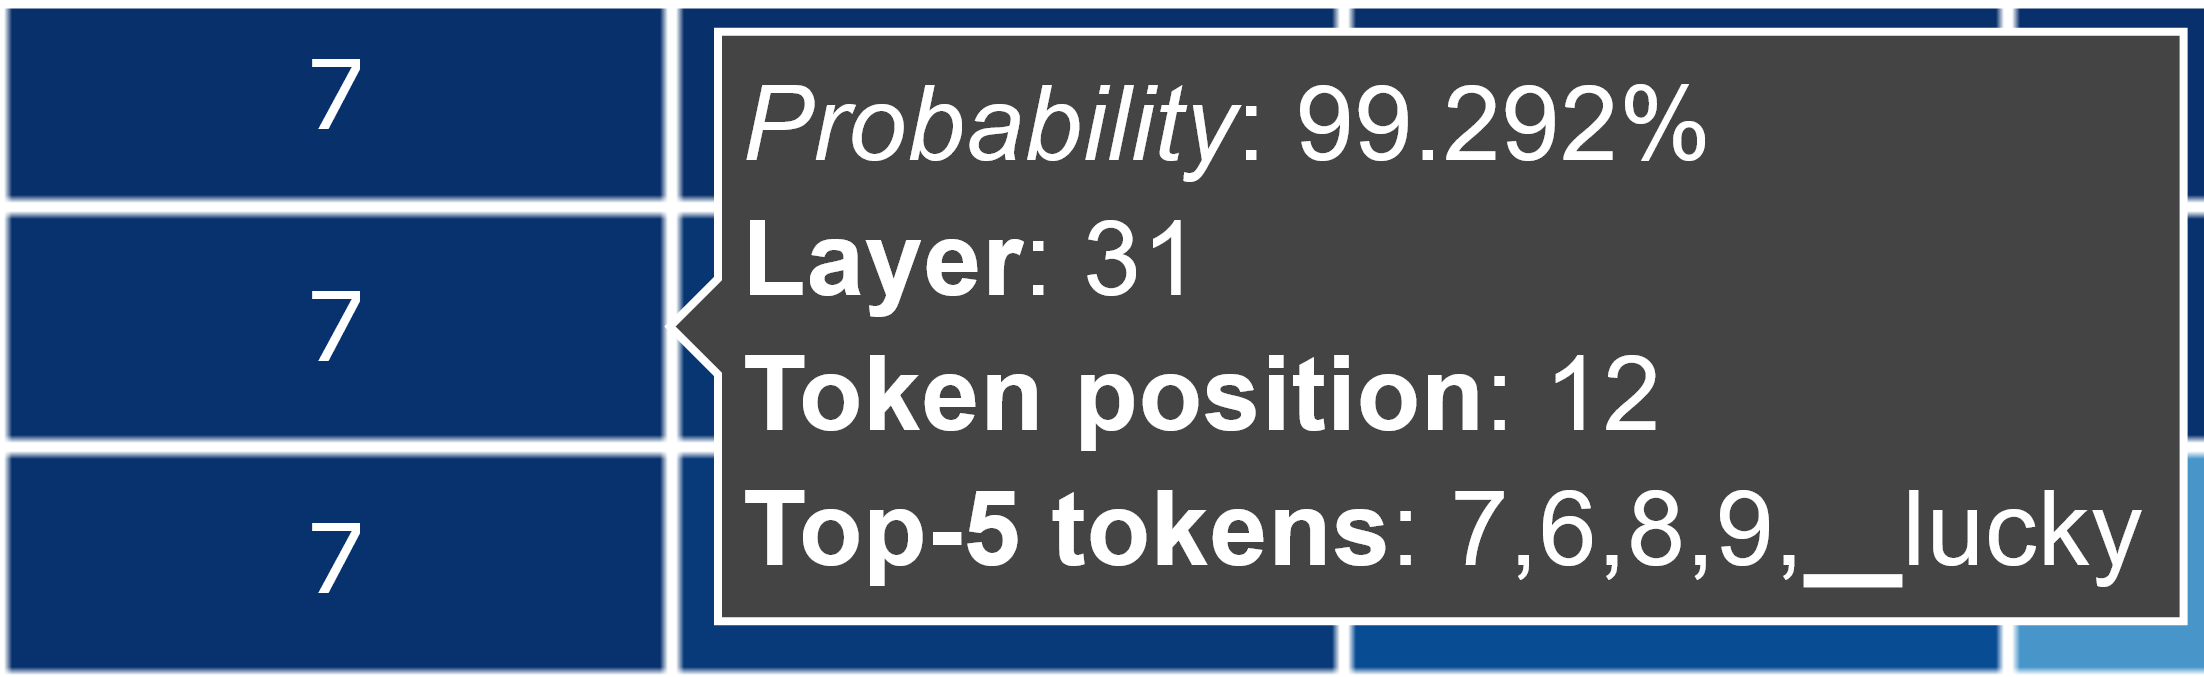
\includegraphics[width=0.4\textwidth]{exp_intravisto_4B_lucky.png}
    %    \end{minipage}
    %\end{frame}

    \section{Embedding Analysis}

    \subsection{Methodology}

    \begin{frame}{Analogy Computation and Evaluation}
        \vspace*{-0.45cm}
        \begin{overlayarea}{\textwidth}{0.5cm}
        \begin{equation*}
            \begin{gathered}
                \only<1>{\textit{king}\,:\,\textit{man}\;=\;\textit{queen}\,:\,\textit{woman}}
                \only<2>{\textit{king}\,-\,\textit{man}\,+\,\textit{woman}\,\approx\,\textit{queen}}
                \only<3>{\text{enc}_{in}({\textit{`king'}})\,-\,\text{enc}_{in}({\textit{`man'}})\,+\,\text{enc}_{in}({\textit{`woman'}})\,\approx\,\text{enc}_{out}({\textit{`queen'}})}
                \only<4>{\gbm{\tilde{w}}\,\approx\,\text{enc}_{out}({\textit{`queen'}})}
            \end{gathered}
        \end{equation*}
        \end{overlayarea}
        \vspace*{0.75cm}
        \begin{minipage}{0.35\textwidth}
            \vspace{-0.35cm}
            \scalebox{0.6}{\parbox{\textwidth}{%
            \begin{equation*}
                \only<3>{\begin{aligned}%
                        {\textit{enc}}_{in}(w) &= 
                        \left\{
                        \begin{array}{cl}
                            \gbm{e}_1^w &\ \text{if}\ \text{`first\_only'} \\
                            \frac{1}{t}\sum_{i=1}^{t}{\gbm{e}_i^w} &\ \text{if}\ \text{`average'} \\
                            \sum_{i=1}^{t}{\gbm{e}_i^w} &\ \text{if}\ \text{`sum'}
                        \end{array}
                        \right. \\[15pt]
                        {\textit{enc}}_{out}(w) &= 
                        \left\{
                        \begin{array}{cl}
                            \{ tok_1^w \} &\ \text{if}\ \text{`first\_only'} \\
                            \{ tok_1^w, \ldots, tok_t^w \} &\ \text{if}\ \text{`subdivide'}
                        \end{array}
                        \right.
                \end{aligned}}
                \only<4>{\begin{aligned}%
                    &\textit{closest}(\gbm{\tilde w}) = \operatornamewithlimits{argmin}_{v \in \mathcal{V}} d_{\textit{dist}}\bigl(\gbm{\tilde w}, \textit{enc}(v)\bigr) \\[17pt]
                    &{\textit{result}\,}^i_j = \Bigl\{\textit{closest}(\gbm{{\tilde w}_i})[\,j\,] \,|\,\forall j = 1,2,\ldots \Bigr\} \\[2pt]
                    &\;\;\;\;\; \forall i = 1,\ldots,n \\[15pt]
                    &\textit{acc}_k\!=\!\frac{1}{n} \sum_{i=1}^{n} \mathbb{I}\Bigl(\!{\left\{ {\textit{result}\,}^i_j \,|\,\forall j = 1,\ldots,k \right\}}\!\cap\!{\textit{sol}\,}^i \neq \emptyset\!\Bigr)
                \end{aligned}}%
            \end{equation*}}}%
        \end{minipage}%
        \begin{minipage}{0.40\textwidth}
            \footnotesize
            \begin{itemize}
                \setlength\itemsep{0.015cm}
                \item<1-1> King/queen analogy in its base form.
                \item<1-1> Solving word analogies showcases an embedding space's ability to model word semantics in a relatively consistent way.
                \item<2-2> Arithmetic resolution of the analogy.
                \item<3-3> Conversion from words to sets of tokens due to the tokenization process of models.
                \item<4-4> Evaluation of the vector representation obtained as the result of embedding arithmetics.
            \end{itemize}
        \end{minipage}%
        \begin{minipage}{0.25\textwidth}
            \begin{overprint}%
                \onslide<1-2>
                \overimage[1cm]{\includegraphics[width=0.65\textwidth]{background_emb-arithmetic_placeholder.pdf}}%
                \onslide<3-4>
                \overimage[0.5cm]{\includegraphics[width=0.72\textwidth]{background_embeddings.pdf}}\overimage[1.6cm]{\includegraphics[width=\textwidth]{pres_drw_input-embedding.pdf}}%
            \end{overprint}%
        \end{minipage}%
    \end{frame}

    \begin{frame}{Dataset and Models}
        \begin{itemize}[<+|visible@+->]
            \item<1-1> Dataset obtained by merging the original \emph{Google analogy dataset} and the \emph{Bigger Analogy Test Set (BATS)} and removing duplicates:
            \begin{itemize}
                \item<1-1> $116 639$ total analogies.
                \item<1-1> $54$ categories.
            \end{itemize}
            \item<2-2> Wide variety of embeddings extrapolated from popular iterations of recent LLMs and older architectures:
            \begin{itemize}
                \item<2-2> \emph{Word2vec} and \emph{GLoVe}.
                \item<2-2> \emph{GPT-2} and \emph{BERT large uncased}.
                \item<2-2> \emph{Llama 2}, \emph{Mistral v0.3} and \emph{Phi 3.5 mini}.
                \item<2-2> \emph{Llama 3} and \emph{Gemma 2}.
            \end{itemize}
            \item<3-3> Experiments that include all types of models use filtered versions of the dataset, where analogies that contain words encoded with multiple tokens are excluded.
        \end{itemize}
    \end{frame}

    \subsection{Results}

    \begin{frame}{Results for Analogies on Input Embeddings (Filtered)}
        \vspace*{0.3cm}
        \begin{minipage}{\textwidth}
            \centering
            \includegraphics[width=0.5\textwidth]{pres_emb-input-l2-l3-m-w2v-g.pdf}%
            \includegraphics[width=0.5\textwidth]{pres_emb-input-g2-p3-b-gpt.pdf}%
        \end{minipage}%
    \end{frame}

    \begin{frame}{Results for Analogies on Input and Output Embeddings}
        \vspace*{0.3cm}
        \begin{minipage}{\textwidth}
            \centering
            \includegraphics[width=0.5\textwidth]{exp_emb_2A_topk_gpt-l2-l3-io.pdf}%
            \includegraphics[width=0.5\textwidth]{exp_emb_2A_topk_gpt-m-p3-io.pdf}%
        \end{minipage}%
    \end{frame}

    %\begin{frame}{Results for Analogies on Interpolated Embeddings}
    %    \vspace*{0.3cm}
    %    \begin{minipage}{\textwidth}
    %        \centering
    %        \includegraphics[width=0.5\textwidth]{exp_emb_2B_topk_l2-7-15-8-io.pdf}%
    %        \includegraphics[width=0.5\textwidth]{exp_emb_2B_topk_m-7-15-8-io.pdf}%
    %    \end{minipage}%
    %\end{frame}

    \section{First Order Prediction}

    \subsection{Methodology}

    \begin{frame}{FOM Computation}
        \begin{minipage}{0.55\textwidth}
            \vspace{0.4cm}
            \footnotesize
            \begin{itemize}[<+|visible@+->]
                \setlength\itemsep{0.35cm}
                \item<1-1> A model of order $0$ can be seen as a probability distribution over the vocabulary, modeling word frequency.
                \item<2-2> On the other hand, a model of order $1$ describes the next-word probability given the previous word.
                \item<3-3> We derive a \emph{First Order Model (FOM)} by removing all intermediate architectural components from an LLM, retaining only the input and output embedding layers along with the residual connections joining them.
                \begin{equation*}
                    \gbm{Q}_{\textit{FOM}} = \operatorname{softmax}(\gbm{Q}_{\textit{FOM}}^{log}) = \operatorname{softmax}(\gbm{W}_{in} \cdot \gbm{W}_{out})
                \end{equation*}
            \end{itemize}
        \end{minipage}%
        \hfill%
        \begin{minipage}{0.4\textwidth}
            \centering
            \begin{overprint}%
                \onslide<1>
                \overimage[1.35cm]{\includegraphics[width=0.98\textwidth]{pres_drw_order-0.pdf}}%
                \onslide<2>
                \overimage[1.35cm]{\includegraphics[width=0.98\textwidth]{pres_drw_order-1.pdf}}%
                \onslide<3>
                \overimage[1.35cm]{\includegraphics[width=0.98\textwidth]{pres_drw_order-1.pdf}}%
                \vspace*{1.4cm}
                \includegraphics[width=0.27\textwidth]{pres_drw_fom.pdf}%
                \includegraphics[width=0.73\textwidth]{pres_drw_embedding.pdf}%
            \end{overprint}%
        \end{minipage}%
    \end{frame}

    \begin{frame}{Reference Transition Matrices}
        \begin{minipage}{0.6\textwidth}
            \begin{itemize}
                \setlength\itemsep{1.4cm}
                \item<1-2> We perform comparisons between the FOM and the identity matrix, modeling the transition matrix of an LLM with tied embeddings.
                \item<2-2> We perform comparisons between the FOM and the transition matrix of an actual Markov model trained using bigrams from the \emph{WikiText 103} dataset.
            \end{itemize}
        \end{minipage}%
        \hfill%
        \begin{minipage}{0.3\textwidth}
            \centering
            \begin{overprint}%
                \onslide<1>
                \overimage[0.7cm]{\includegraphics[width=0.8\textwidth]{pres_drw_trans-i.pdf}}%
                \onslide<2>
                \overimage[0.7cm]{\includegraphics[width=0.8\textwidth]{pres_drw_trans-i.pdf}}%
                \overimage[2.5cm]{\hspace*{-0.95cm}\includegraphics[width=\textwidth]{pres_drw_trans-markov.pdf}}%
            \end{overprint}%
        \end{minipage}%
    \end{frame}

    \begin{frame}{Evaluation Metrics}
        \begin{minipage}{0.45\textwidth}
            \begin{itemize}[<+|visible@+->]
                \setlength\itemsep{0.3cm}
                \item<1-1> We start by performing a \emph{naïve direct comparison} between transition matrices.
                \item<2-2> Followed by the use of \emph{set similarity metrics} (such as top-$k$ accuracy, Jaccard similarity and overlap coefficient) to obtain more reliable estimates.
                \item<3-3> We end with the computation of \emph{probabilistic metrics} such as perplexity and KL divergence.
            \end{itemize}
        \end{minipage}%
        \begin{minipage}{0.55\textwidth}
            \begin{equation*}
                \uncover<+|visible@1+->{%
                    \left\{
                        \begin{array}{cl}
                            d_{\textit{FOM},I} &= \| \gbm{Q}_{\textit{FOM}} - \gbm{I}_V \|_F \\
                            d_{\textit{FOM},\textit{markov}} &= \| \gbm{Q}_{\textit{FOM}} - \gbm{Q}_{\textit{markov}} \|_F
                        \end{array}
                    \right.
                }
            \end{equation*}
            \scalebox{0.82}{\parbox{\textwidth}{%
            \begin{equation*}
                \begin{gathered}
                \uncover<+|visible@2+->{%
                    \;\;\;\textit{acc}_{k_1,k_2}(\gbm{Q}_1, \gbm{Q}_2) = \frac{1}{|\mathcal{V}|} \sum_{v \in \mathcal{V}}{\textit{tok\_overlap}_{k_1,k_2}(\gbm{Q}_1, \gbm{Q}_2, v)}
                }
                \end{gathered}
            \end{equation*}}}
            \vspace*{-0.2cm}
            \scalebox{0.9}{\parbox{\textwidth}{%
            \begin{equation*}
                \begin{gathered}
                    \uncover<+|visible@3+->{%
                        PP(\gbm{Q}, S) = e^{-\frac{1}{T}\sum_{t=1}^{T}{\ln{\left((\gbm{Q})_{S(t-1),S(t)}\right)}}} \\[10pt]
                        \ D_{KL}^v(\gbm{Q}_{ref} || \gbm{Q}_{model})\!=\!\sum_{w \in \mathcal{V}}{\!\bigl((\gbm{Q}_{ref})_{v,w}\bigr)\ln{\frac{(\gbm{Q}_{ref})_{v,w}}{(\gbm{Q}_{model})_{v,w}}}}
                    }
                \end{gathered}
            \end{equation*}}}
        \end{minipage}%
    \end{frame}

    %\begin{equation*}
    %    \begin{gathered}
    %        \textit{accuracy}_{k_1,k_2}(\gbm{Q}_1, \gbm{Q}_2) = \frac{1}{V} \sum_{v \in \mathcal{V}}{\textit{tok\_overlap}_{k_1,k_2}(\gbm{Q}_1, \gbm{Q}_2, v)} \\
    %        \textit{tok\_overlap}_{k_1,k_2}(\gbm{Q}_1, \gbm{Q}_2, v) = \left\{
    %            \begin{array}{cl}
    %                1 &\ \text{if}\ \operatorname{top-k}(\gbm{Q}_1, k_1, v) \cap \operatorname{top-k}(\gbm{Q}_2, k_2, v) \neq \emptyset \\
    %                0 &\ \text{otherwise}
    %            \end{array}
    %            \right.
    %        \begin{aligned}
    %            \operatorname{overlap}_k(\gbm{Q}_1, \gbm{Q}_2) &= \frac{1}{V}\sum_{v \in \mathcal{V}}{\frac{|\operatorname{top-k}(\gbm{Q}_1, k, v) \cap \operatorname{top-k}(\gbm{Q}_2, k, v)|}{\operatornamewithlimits{min}\bigl\{|\operatorname{top-k}(\gbm{Q}_1, k, v)|, |\operatorname{top-k}(\gbm{Q}_2, k, v)|\bigr\}}} \\
    %            \operatorname{J}_k(\gbm{Q}_1, \gbm{Q}_2) &= \frac{1}{V}\sum_{v \in \mathcal{V}}{\frac{|\operatorname{top-k}(\gbm{Q}_1, k, v) \cap \operatorname{top-k}(\gbm{Q}_2, k, v)|}{|\operatorname{top-k}(\gbm{Q}_1, k, v) \cup \operatorname{top-k}(\gbm{Q}_2, k, v)|}} \\
    %        \end{aligned}
    %    \end{gathered}
    %\end{equation*}

    \subsection{Results}
    %\begin{frame}{}
    %    \begin{minipage}{\textwidth}
    %        \centering
    %        \includegraphics[width=0.3\textwidth]{exp_fom_1A_l2-topk-markov.pdf}%
    %        \includegraphics[width=0.3\textwidth]{exp_fom_1A_m-topk-markov.pdf}%
    %        \includegraphics[width=0.3\textwidth]{exp_fom_1A_p-topk-markov.pdf}%
    %    \end{minipage}%

    %    \begin{minipage}{\textwidth}
    %        \vspace{-0.2cm}
    %        \centering
    %        \includegraphics[width=0.3\textwidth]{exp_fom_1A_l2-topk-id.pdf}%
    %        \includegraphics[width=0.3\textwidth]{exp_fom_1A_m-topk-id.pdf}%
    %        \includegraphics[width=0.3\textwidth]{exp_fom_1A_p-topk-id.pdf}%
    %    \end{minipage}%
    %\end{frame}

    \begin{frame}{Results for Direct Comparison}
        \begin{minipage}{\textwidth}
            \centering
            \vspace*{-0.15cm}
            \hspace*{-0.2cm}
            \begin{tikzpicture}
                \node (table1) at (0,0) {
                    \resizebox{0.5\textwidth}{!}{%
                    \begin{tabular}{| c | c c c |}
                        \rowcolorhang{bluePolimi!70!white}
                        \hline
                        \textbf{Distance} & $\textbf{d(FOM, I)}$ & $\textbf{d(FOM, Markov)}$ & $\textbf{d(Markov, I)}$ \\
                        \hline \hline
                            \textbf{Llama 2} & $178.88$ & $6.37$ & $178.99$ \\[2px]
                            \textbf{Llama 2 with RMS} & $180.33$ & $23.13$ & '' \\[2px]
                            \textbf{Mistral} & $181.02$ & $5.95$ & $181.11$ \\[2px]
                            \textbf{Mistral with RMS} & $180.99$ & $6.07$ & '' \\[2px]
                            \textbf{Phi 3.5} & $179.06$ & $6.30$ & $179.16$ \\[2px]
                            \textbf{Phi 3.5 with RMS} & $201.15$ & $91.53$ & '' \\[2px]
                        \hline
                    \end{tabular}
                    }%
                };
                \node (table2) at (7.6,0) {
                    \resizebox{0.5\textwidth}{!}{%
                    \begin{tabular}{| c | c c c c |}
                        \rowcolorhang{bluePolimi!70!white}
                        \hline
                        & \textbf{Identity} & \textbf{Markov} & \textbf{Identity} & \textbf{Markov} \\[-0.2pt]
                        \rowcolorhang{bluePolimi!70!white}
                        \multirow{-2}{*}{\textbf{FOM Top-k Accuracy}} & $\gbm{k=5}$ & $\gbm{k_1=5, k_2=1}$ & $\gbm{k=50}$ & $\gbm{k_1=50, k_2=1}$ \\
                        \hline \hline
                            \textbf{Llama 2} & $.0011$ & $.0624$ & $.0055$ & $.1120$ \\[2px]
                            \textbf{Llama 2 with RMS} & $.0010$ & $.0616$ & $.0056$ & $.1105$ \\[2px]
                            \textbf{Mistral} & $.0534$ & $.0061$ & $.1308$ & $.0204$ \\[2px]
                            \textbf{Mistral with RMS} & $.0543$ & $.0044$ & $.1323$ & $.0163$ \\[2px]
                            \textbf{Phi 3.5} & $.0002$ & $.0482$ & $.0016$ & $.0926$ \\[2px]
                            \textbf{Phi 3.5 with RMS} & $.0002$ & $.0479$ & $.0017$ & $.0917$ \\[2px]
                        \hline
                    \end{tabular}
                    }
                };
                \only<2>{\draw[color=red,thick] (10.14,0.36) rectangle (10.8,0.6);}
                \only<2>{\draw[color=red,thick] (8.82,-0.22) rectangle (9.48,0.02);}
                \only<2>{\draw[color=red,thick] (10.14,-0.8) rectangle (10.8,-0.56);}
            \end{tikzpicture}
        \end{minipage}%

        \vspace{-0.2cm}%
        \begin{minipage}{0.33\textwidth}%
            \centering%
            \begin{tikzpicture}
                \node[inner sep=0] (img) {\includegraphics[width=0.98\textwidth]{exp_fom_1B_l2-opmetrics.pdf}};
                \node[anchor=south] at ([xshift=0.2cm, yshift=-0.15cm]img.north) {\tiny Llama 2};
            \end{tikzpicture}%
        \end{minipage}%
        \begin{minipage}{0.33\textwidth}%
            \centering%
            \begin{tikzpicture}
                \node[inner sep=0] (img) {\includegraphics[width=0.98\textwidth]{pres_opmetrics-m.pdf}};
                \node[anchor=south] at ([xshift=0.2cm, yshift=-0.15cm]img.north) {\tiny Mistral};
            \end{tikzpicture}%
        \end{minipage}%
        \begin{minipage}{0.33\textwidth}%
            \centering%
            \begin{tikzpicture}
                \node[inner sep=0] (img) {\includegraphics[width=0.98\textwidth]{pres_opmetrics-p.pdf}};
                \node[anchor=south] at ([xshift=0.2cm, yshift=-0.15cm]img.north) {\tiny Phi 3.5};
            \end{tikzpicture}%
        \end{minipage}%
    \end{frame}

    \begin{frame}{Results for Probabilistic Comparison}
        \hspace{-0.4cm}%
        \begin{minipage}{0.75\textwidth}
            \centering
            \includegraphics[width=\textwidth]{exp_fom_2A_l2-perpdens-owt.pdf}%
        \end{minipage}%
        \begin{minipage}{0.25\textwidth}
            \centering
            \vspace{-0.2cm}
            {\hspace{0.8cm} \scriptsize Llama 2 \\[15pt]}
            \begin{tikzpicture}
                \useasboundingbox (-1.31, -1) rectangle (0.59,1); 
                \node (table) {
                    \setlength{\tabcolsep}{2pt}%
                    \resizebox{1.19\columnwidth}{!}{%
                    \begin{tabular}{| >{\columncolor{bluePolimi!70!white}}c || c c c c |}
                        \hhline{-||----}
                        \rowcolorhang{bluePolimi!70!white}
                            \textbf{Llama 2} $\gbm{{{\bar D}_{KL}}}$ & \textbf{FOM} & \makecell{\textbf{FOM}\\\textbf{with RMS}} & \Gape[0pt][1pt]{\makecell{\textbf{Markov}\\\textbf{model}}} & \Gape[0pt][1pt]{\makecell{\textbf{Identity}\\\textbf{matrix}}} \\
                        \hhline{=::====}
                        \textbf{FOM} & $-$ & $-$ & $0.05469$ & $17.26026$ \\[2px]
                        \textbf{FOM with RMS} & $-$ & $-$ & $2.09969$ & $19.60988$ \\[2px]
                        \textbf{Markov model} & $0.20263$ & $2.26218$ & $-$ & $17.45812$ \\[2px]
                        \textbf{Identity matrix} & $10.37378$ & $12.41667$ & $10.38829$ & $-$ \\[2px]
                        \hhline{-||----}
                    \end{tabular}%
                    }
                };
                \only<2>{\draw[color=red,thick] (-0.8,-0.45) rectangle (-0.12,-0.24);}
                \only<2>{\draw[color=red,thick] (0.82,0.05) rectangle (1.5,0.27);}
            \end{tikzpicture}
        \end{minipage}

        \hspace{-0.4cm}%
        \begin{minipage}{0.75\textwidth}
            \centering
            \includegraphics[width=\textwidth]{exp_fom_2A_m-perpdens-owt.pdf}%
        \end{minipage}%
        \begin{minipage}{0.25\textwidth}
            \centering
            \vspace{-0.2cm}
            {\hspace{0.8cm} \scriptsize Mistral \\[15pt]}
            \begin{tikzpicture}
                \useasboundingbox (-1.31, -1) rectangle (0.59,1); 
                \node (table) {
                    \setlength{\tabcolsep}{2pt}%
                    \resizebox{1.19\columnwidth}{!}{%
                    \begin{tabular}{| >{\columncolor{bluePolimi!70!white}}c || c c c c |}
                        \hhline{-||----}
                        \rowcolorhang{bluePolimi!70!white}
                            \textbf{Mistral} $\gbm{{{\bar D}_{KL}}}$ & \textbf{FOM} & \makecell{\textbf{FOM}\\\textbf{with RMS}} & \Gape[0pt][1pt]{\makecell{\textbf{Markov}\\\textbf{model}}} & \Gape[0pt][1pt]{\makecell{\textbf{Identity}\\\textbf{matrix}}} \\
                        \hhline{=::====}
                        \textbf{FOM} & $-$ & $-$ & $0.07512$ & $17.65959$ \\[2px]
                        \textbf{FOM with RMS} & $-$ & $-$ & $0.45097$ & $17.64404$ \\[2px]
                        \textbf{Markov model} & $0.16343$ & $0.56115$ & $-$ & $17.41740$ \\[2px]
                        \textbf{Identity matrix} & $10.37500$ & $9.55581$ & $10.40969$ & $-$ \\[2px]
                        \hhline{-||----}
                    \end{tabular}%
                    }
                };
                \only<2>{\draw[color=red,thick] (-0.8,-0.45) rectangle (-0.12,-0.24);}
                \only<2>{\draw[color=red,thick] (0.82,0.05) rectangle (1.5,0.27);}
            \end{tikzpicture}
        \end{minipage}
    \end{frame}

    \section{Conclusions}

    \begin{frame}{Main Contributions and Future Developments}
        \begin{itemize}[<+|visible@+->]
            \item<1-1> Main contributions:
            \begin{itemize}
                \item<1-1> Creation of a visualization tool for internal states of transformer-based LMs.
                \item<1-1> Reconfirmed linear properties of embedding spaces for larger transformer architectures.
                \item<1-1> Confirmed general tendency of FOMs to model bigram statistics over the vocabulary for LLMs.
            \end{itemize}
            \item<2-2> Possible future developments:
            \begin{itemize}
                \item<2-2> Extend InTraVisTo by adding support for new \emph{decoding techniques}, \emph{model architectures} and \emph{injection approaches}.
                \item<2-2> Investigate the possibility of utilizing the transition matrix of a Markov model to initialize the embedding or unembedding weights for model training.
            \end{itemize}
        \end{itemize}
    \end{frame}

    \begin{frame}[plain]{}
        \vspace{1.5cm}
        \begin{minipage}[t][\baselineskip]{\textwidth}
        {
            \center
            \Large\bf Thank You for Your Attention! \par
        }
        \end{minipage}
    \end{frame}

    \section{}

    \begin{frame}{References}
        \footnotesize
        \begin{itemize}
            \item Slides $4$, $20$: \url{https://developers.google.com/machine-learning/crash-course/embeddings/embedding-space}.
            \item Slide $6$:
            \begin{itemize}
                \item nostalgebraist. interpreting gpt: the logit lens, 2020. URL \url{https://www.alignmentforum.org/posts/AcKRB8wDpdaN6v6ru/interpreting-gpt-the-logit-lens}.
                \item I. Tufanov, K. Hambardzumyan, J. Ferrando, and E. Voita. LM transparency tool: Interactive tool for analyzing transformer language models. CoRR, abs/2404.07004,2024. doi: 10.48550/ARXIV.2404.07004. URL \url{https://doi.org/10.48550/arXiv.2404.07004}.
            \end{itemize}
            \item InTraVisTo: \url{https://github.com/daviderigamonti/InTraVisTo}.
            \item Thesis Repository: \url{https://github.com/daviderigamonti/NLP-Thesis}.
        \end{itemize}
    \end{frame}

\end{document}
